% !TEX root = ../Thesis.tex
\chapter{Laser Induced Decoherence}

In this chapter I will address the results gained so far. Looking first at the impact of laser illumination on coherence times before examining the impact of the Stark shift on selenium donors in purified silicon and the hyperfine coupling of phosphorus donors to $^{29}$Si nuclei in natural silicon.

\section{Illumination Induced Decoherence}

\subsection{Initial Measurements}

The first step undertaken before any laser illumination occurs is to characterise the sample's $T_1$ and $T_2$ times `in the dark' at the measurement temperature.
Experiments were performed at 8~K and 7k, with typical $T_1$ and $T_2$ decays shown in figure \ref{fig:t1andt2}.
The inversion recovery has been fitted with a standard exponential decay whilst the $T_2$ decay has had a stretched exponential decay applied.
The time constants of these decays give the $T_1$ and $T_2$ times with errors in the fit used to establish errors in their values.
The stretched exponential decay of $T_2$ indicates the presence of spectral diffusion.
$T_2$ decays with dynamical decoupling applied do not have this stretch factor as they are isolated from spectral diffusion.
A problem with the results presented here is a variation in the time constant for the decay in the dark, with 2.8~ms found in the high power experiments, whilst 6.4~ms was found during the low power experiments.
According to simulations and literature results this difference in $T_1$ would correspond to a temperature difference of approximately 0.3~K \cite{Tyryshkin2012}.
These results are therefore presented separately to avoid confusion.
It is possible that this is attributable to different flow rates in the helium cryostat, meaning that use of a dry cryostat, which offers much greater temperature precision, would be beneficial.
At 7~K $T_1$ was $32\pm0.1$ms and $T_2$ was unchanged.


\begin{figure}
\centering
\begin{subfigure}[b]{0.5\textwidth}
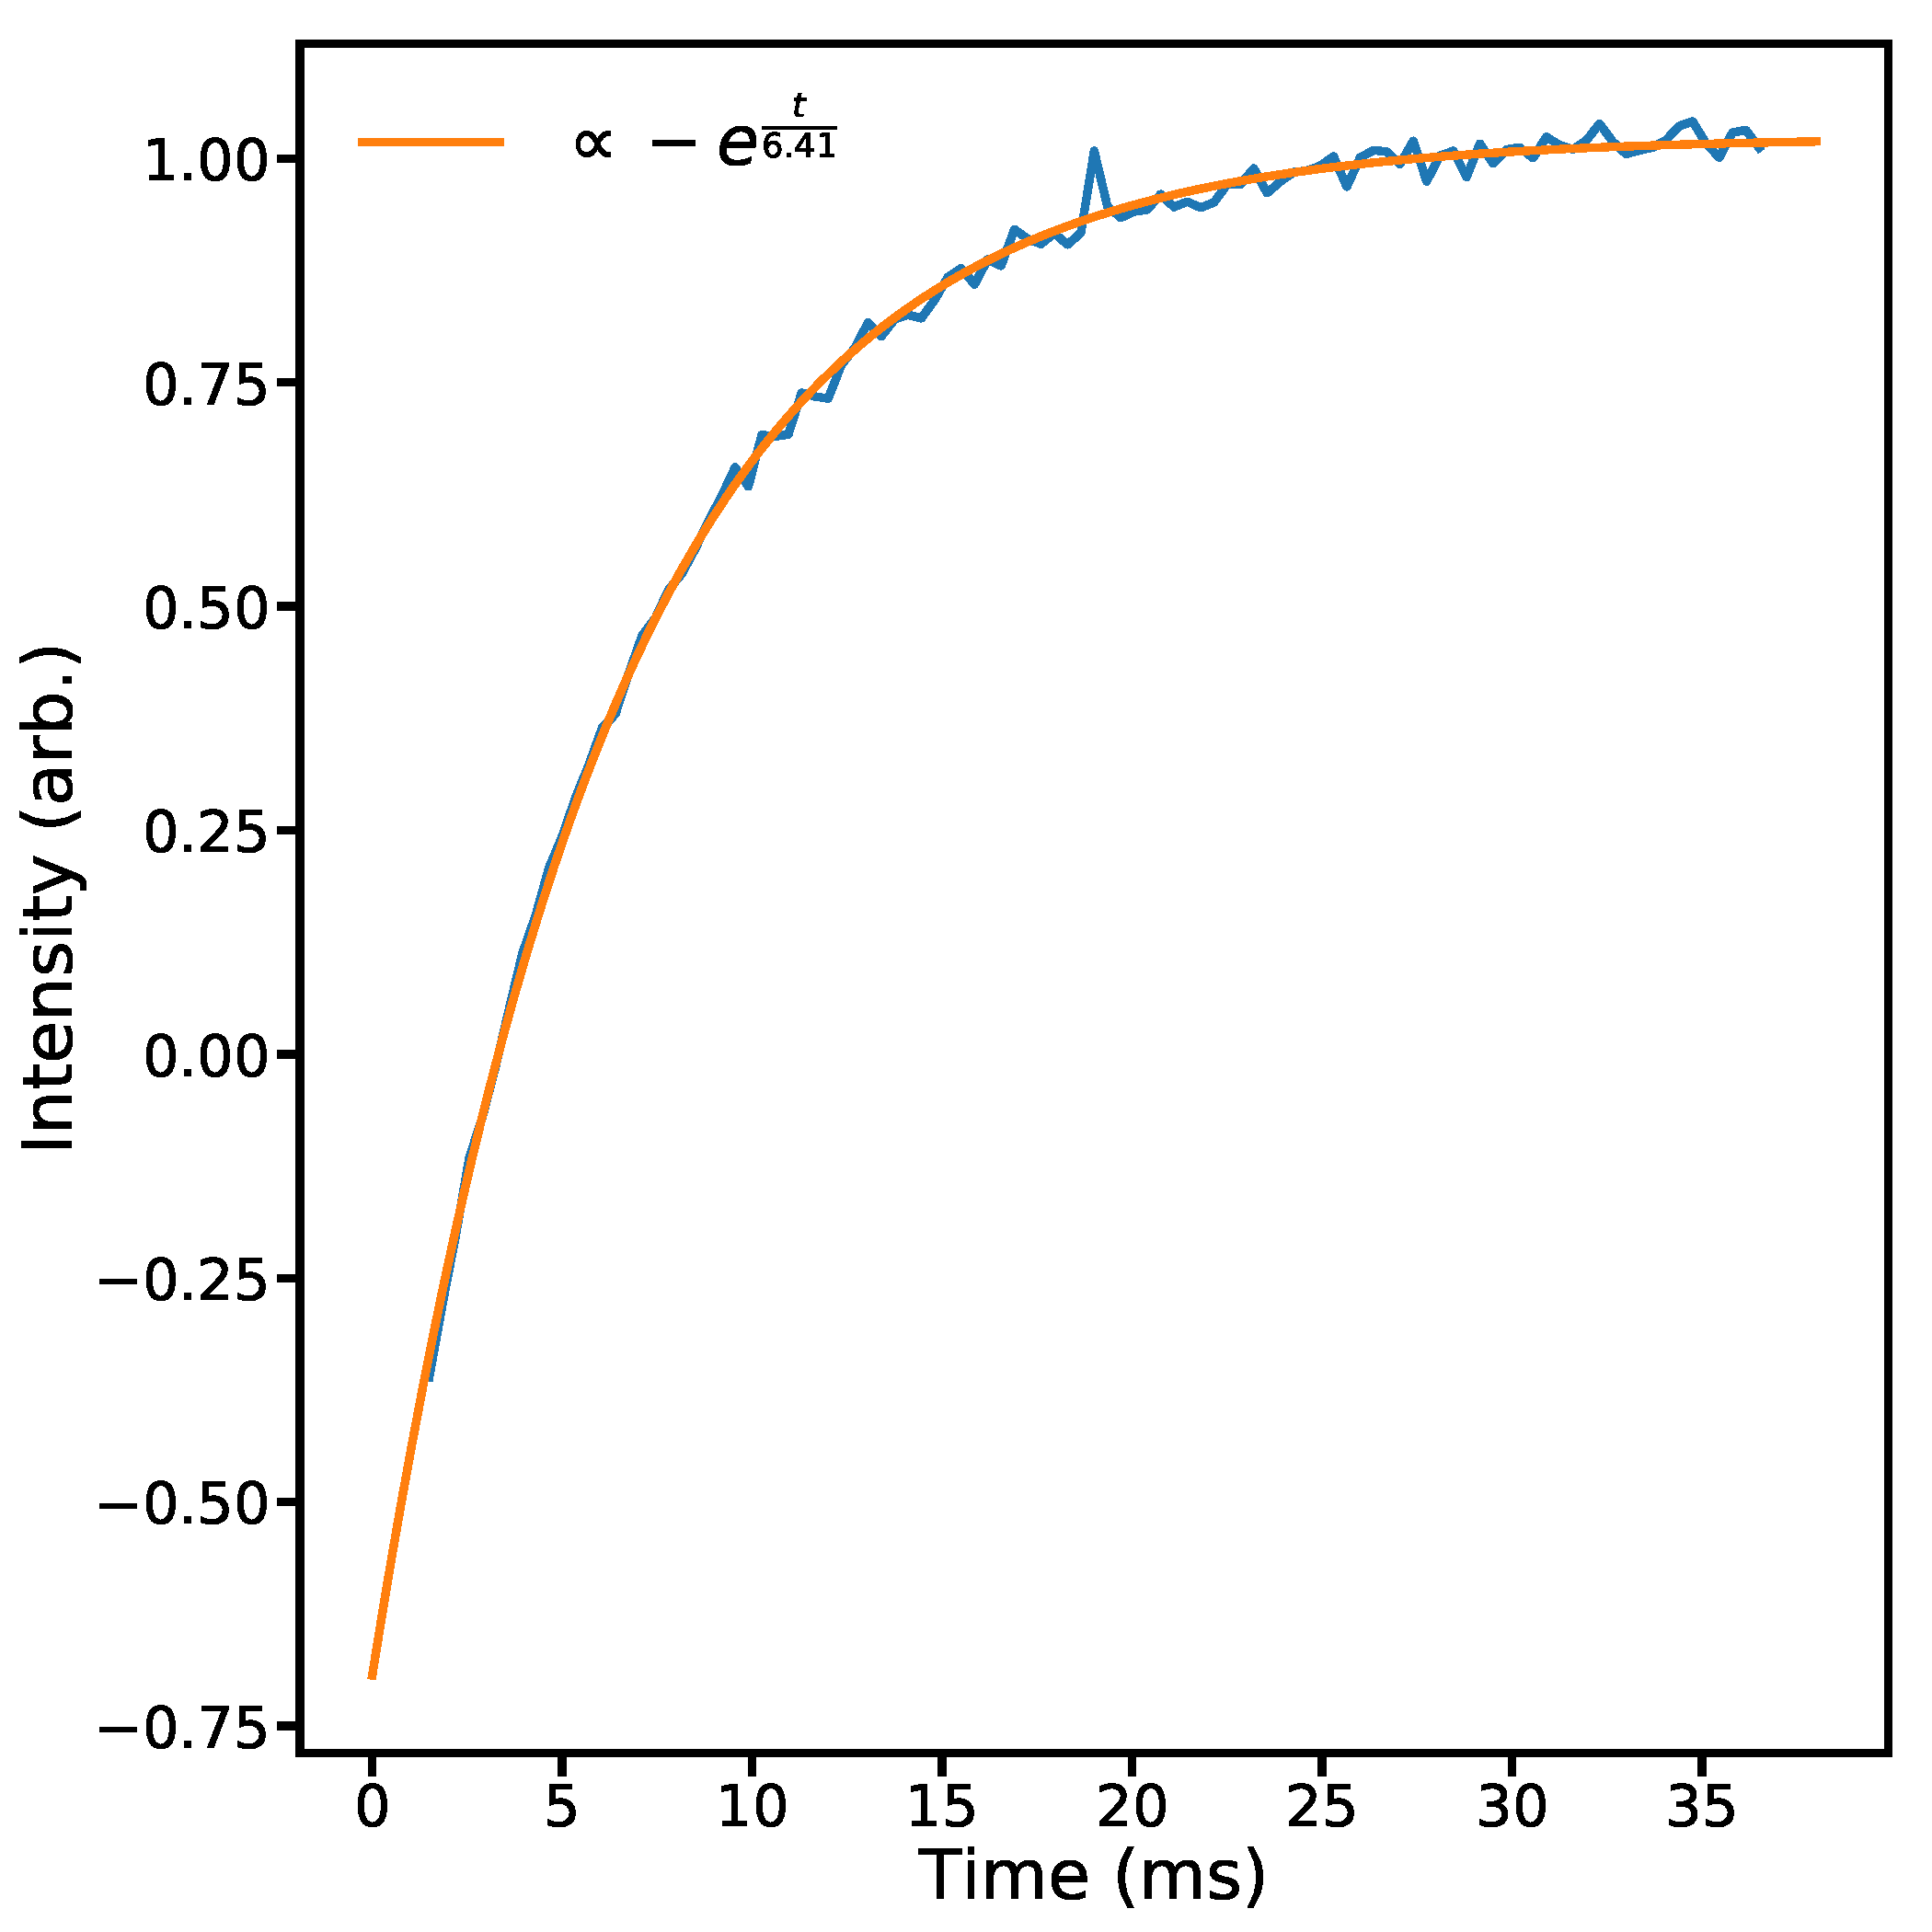
\includegraphics[width=\columnwidth]{Figures/T1Dark.pdf}{(a)}
\end{subfigure}%
\begin{subfigure}[b]{0.5\textwidth}
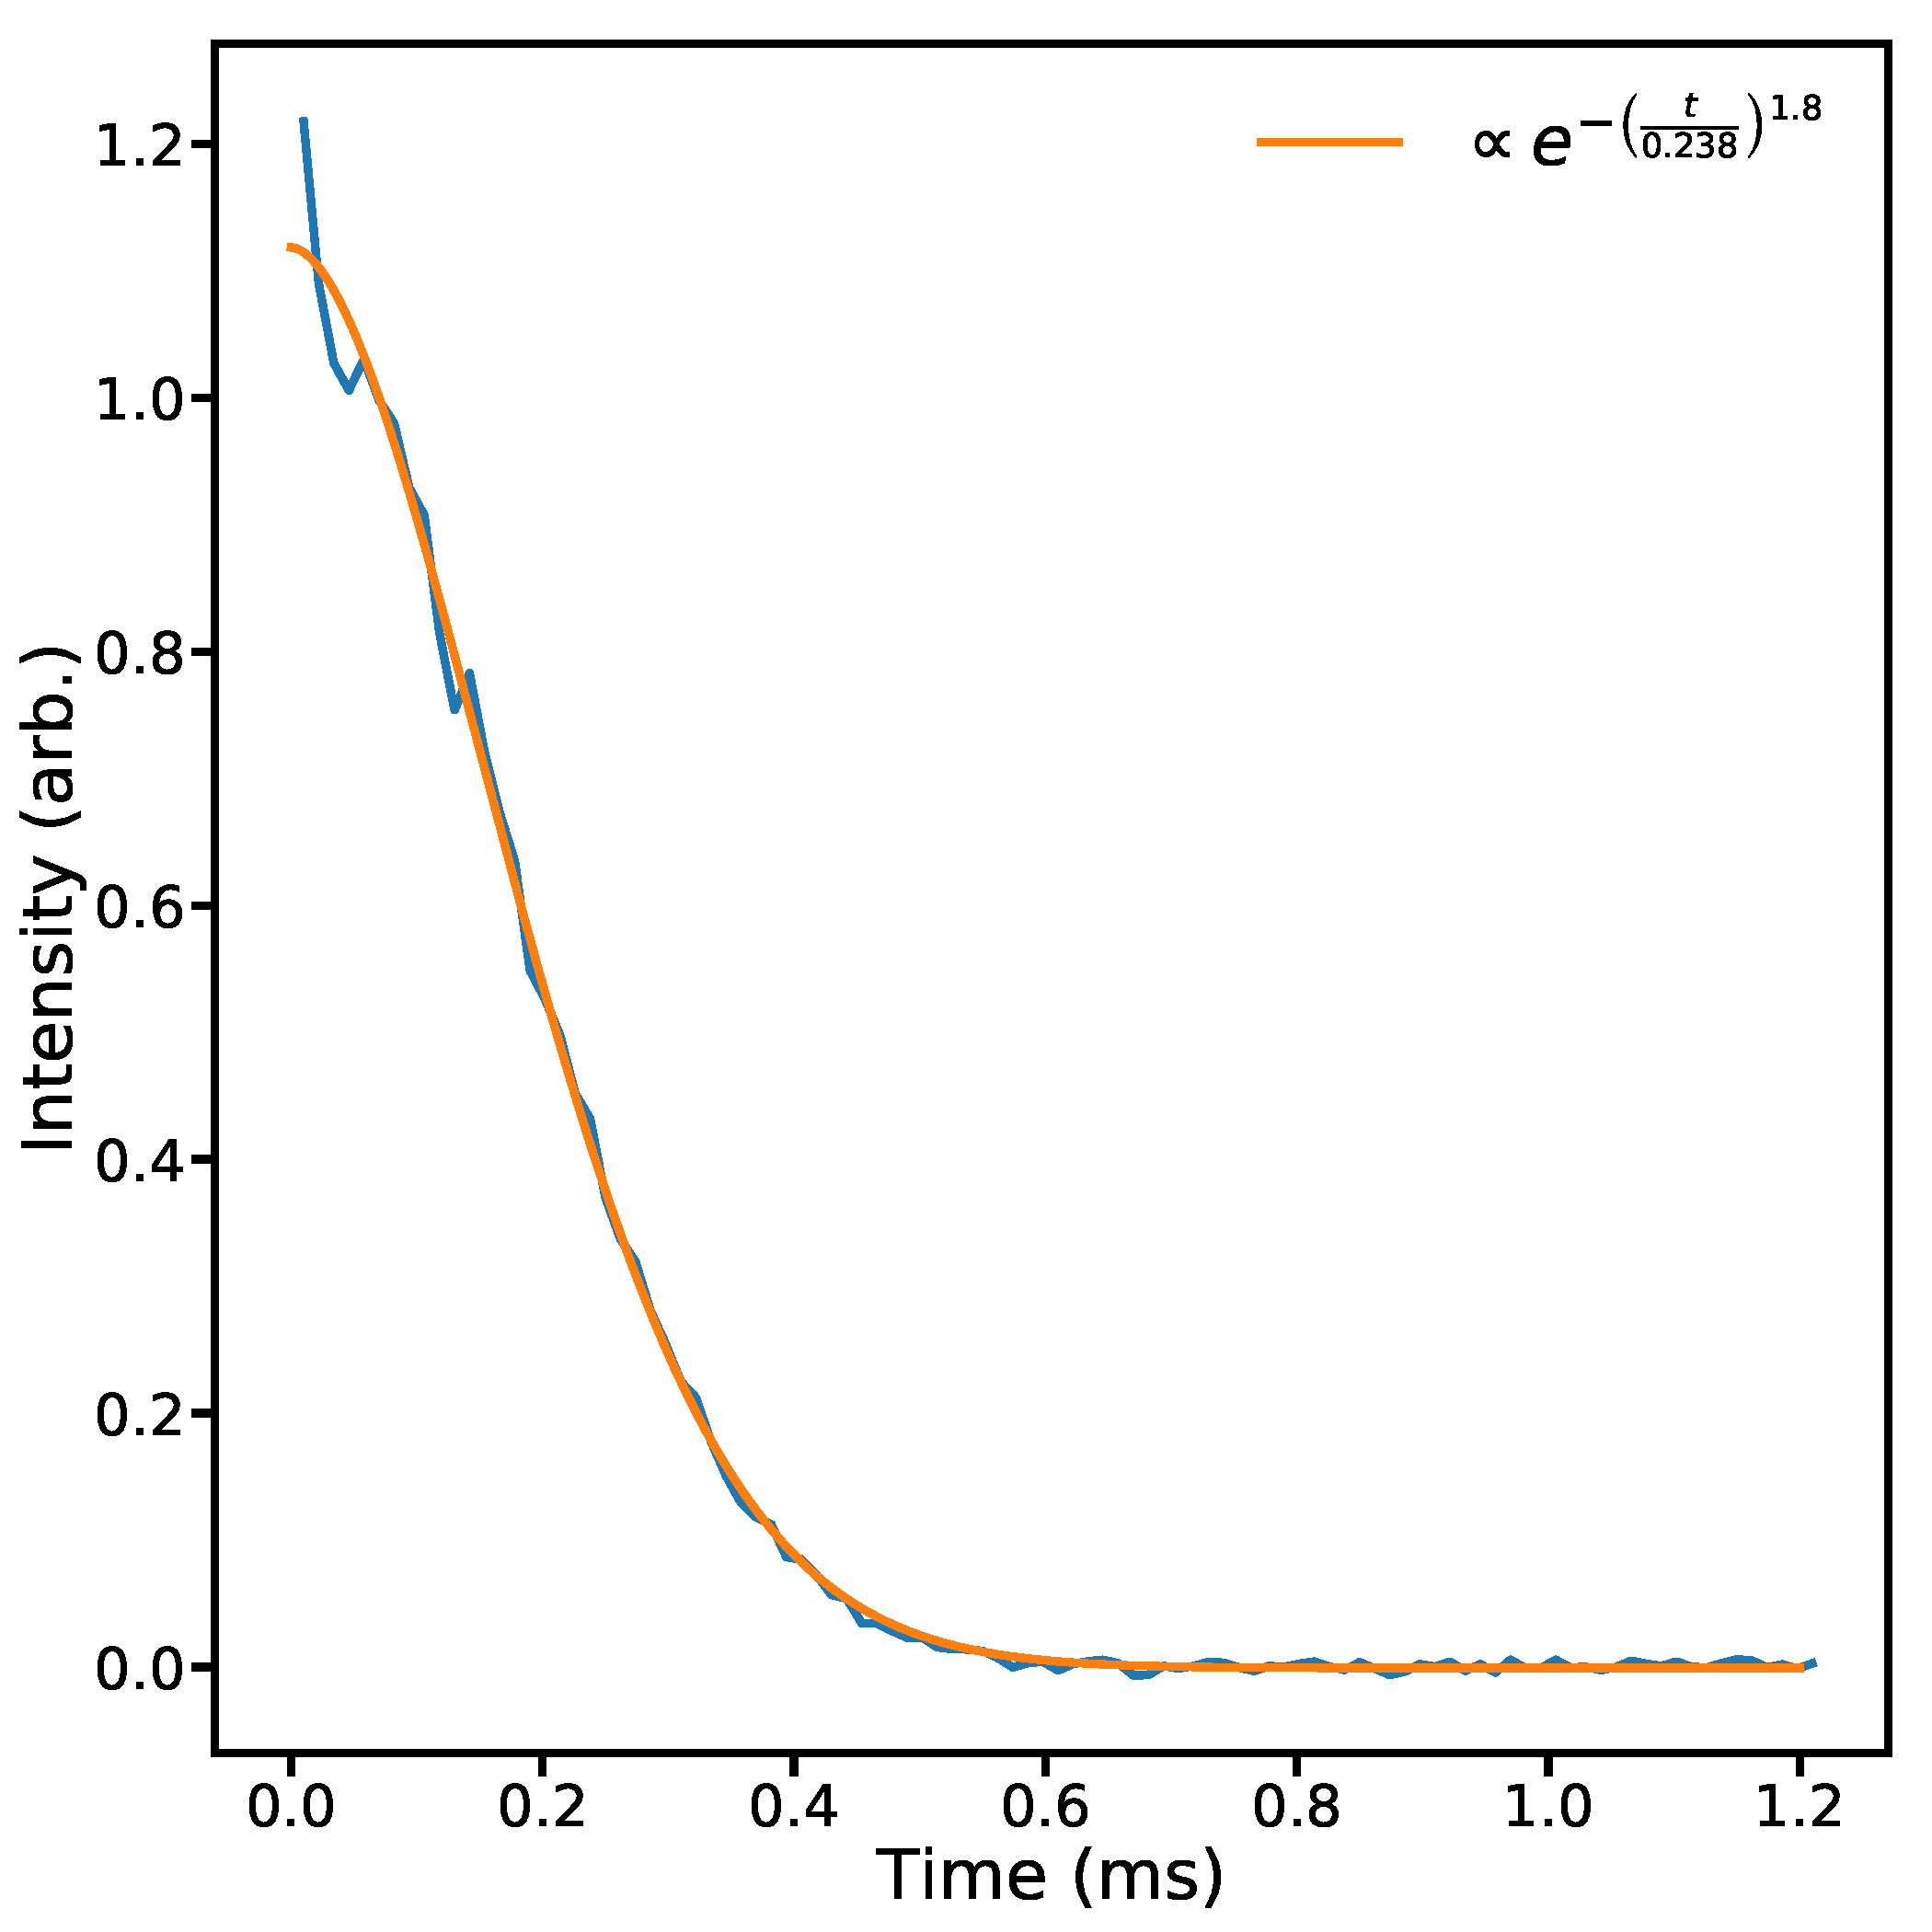
\includegraphics[width=\columnwidth]{Figures/T2Dark.pdf}{(b)}
\end{subfigure}%
\caption[$T_1$ and $T_2$ decays]{Typical $T_1$ and $T_2$ decays showing the inversion recovery for $T_1$ and the characteristic stretched exponential for $T_2$, indicating the presence of spectral diffusion.}
\label{fig:t1andt2}
\end{figure}

\subsection{Bi-Exponential Inversion Recovery}

A set of high power measurements have been taken at powers between 2~mW and 130~mW, at wavelengths 1058~nm, 1070~nm and 1080~nm, and at temperatures of 7~K and 8k.
At each power and wavelength 3 measurements were made: $T_1$, $T_2$ and $T_2$ whilst using a 4 $\pi$ pulse dynamical decoupling sequence - CPMG-4 \cite{Carr1954}.
An initial observation is that the inversion recovery is best fit by a bi-exponential (rather than a single exponential) of the form:

\begin{equation}
a e^{\frac{t}{T_{1a}}} + b e^{\frac{t}{T_{1b}}}
\end{equation}

this is clearly seen in figure \ref{fig:biexpDec}.

\begin{figure}
\centering
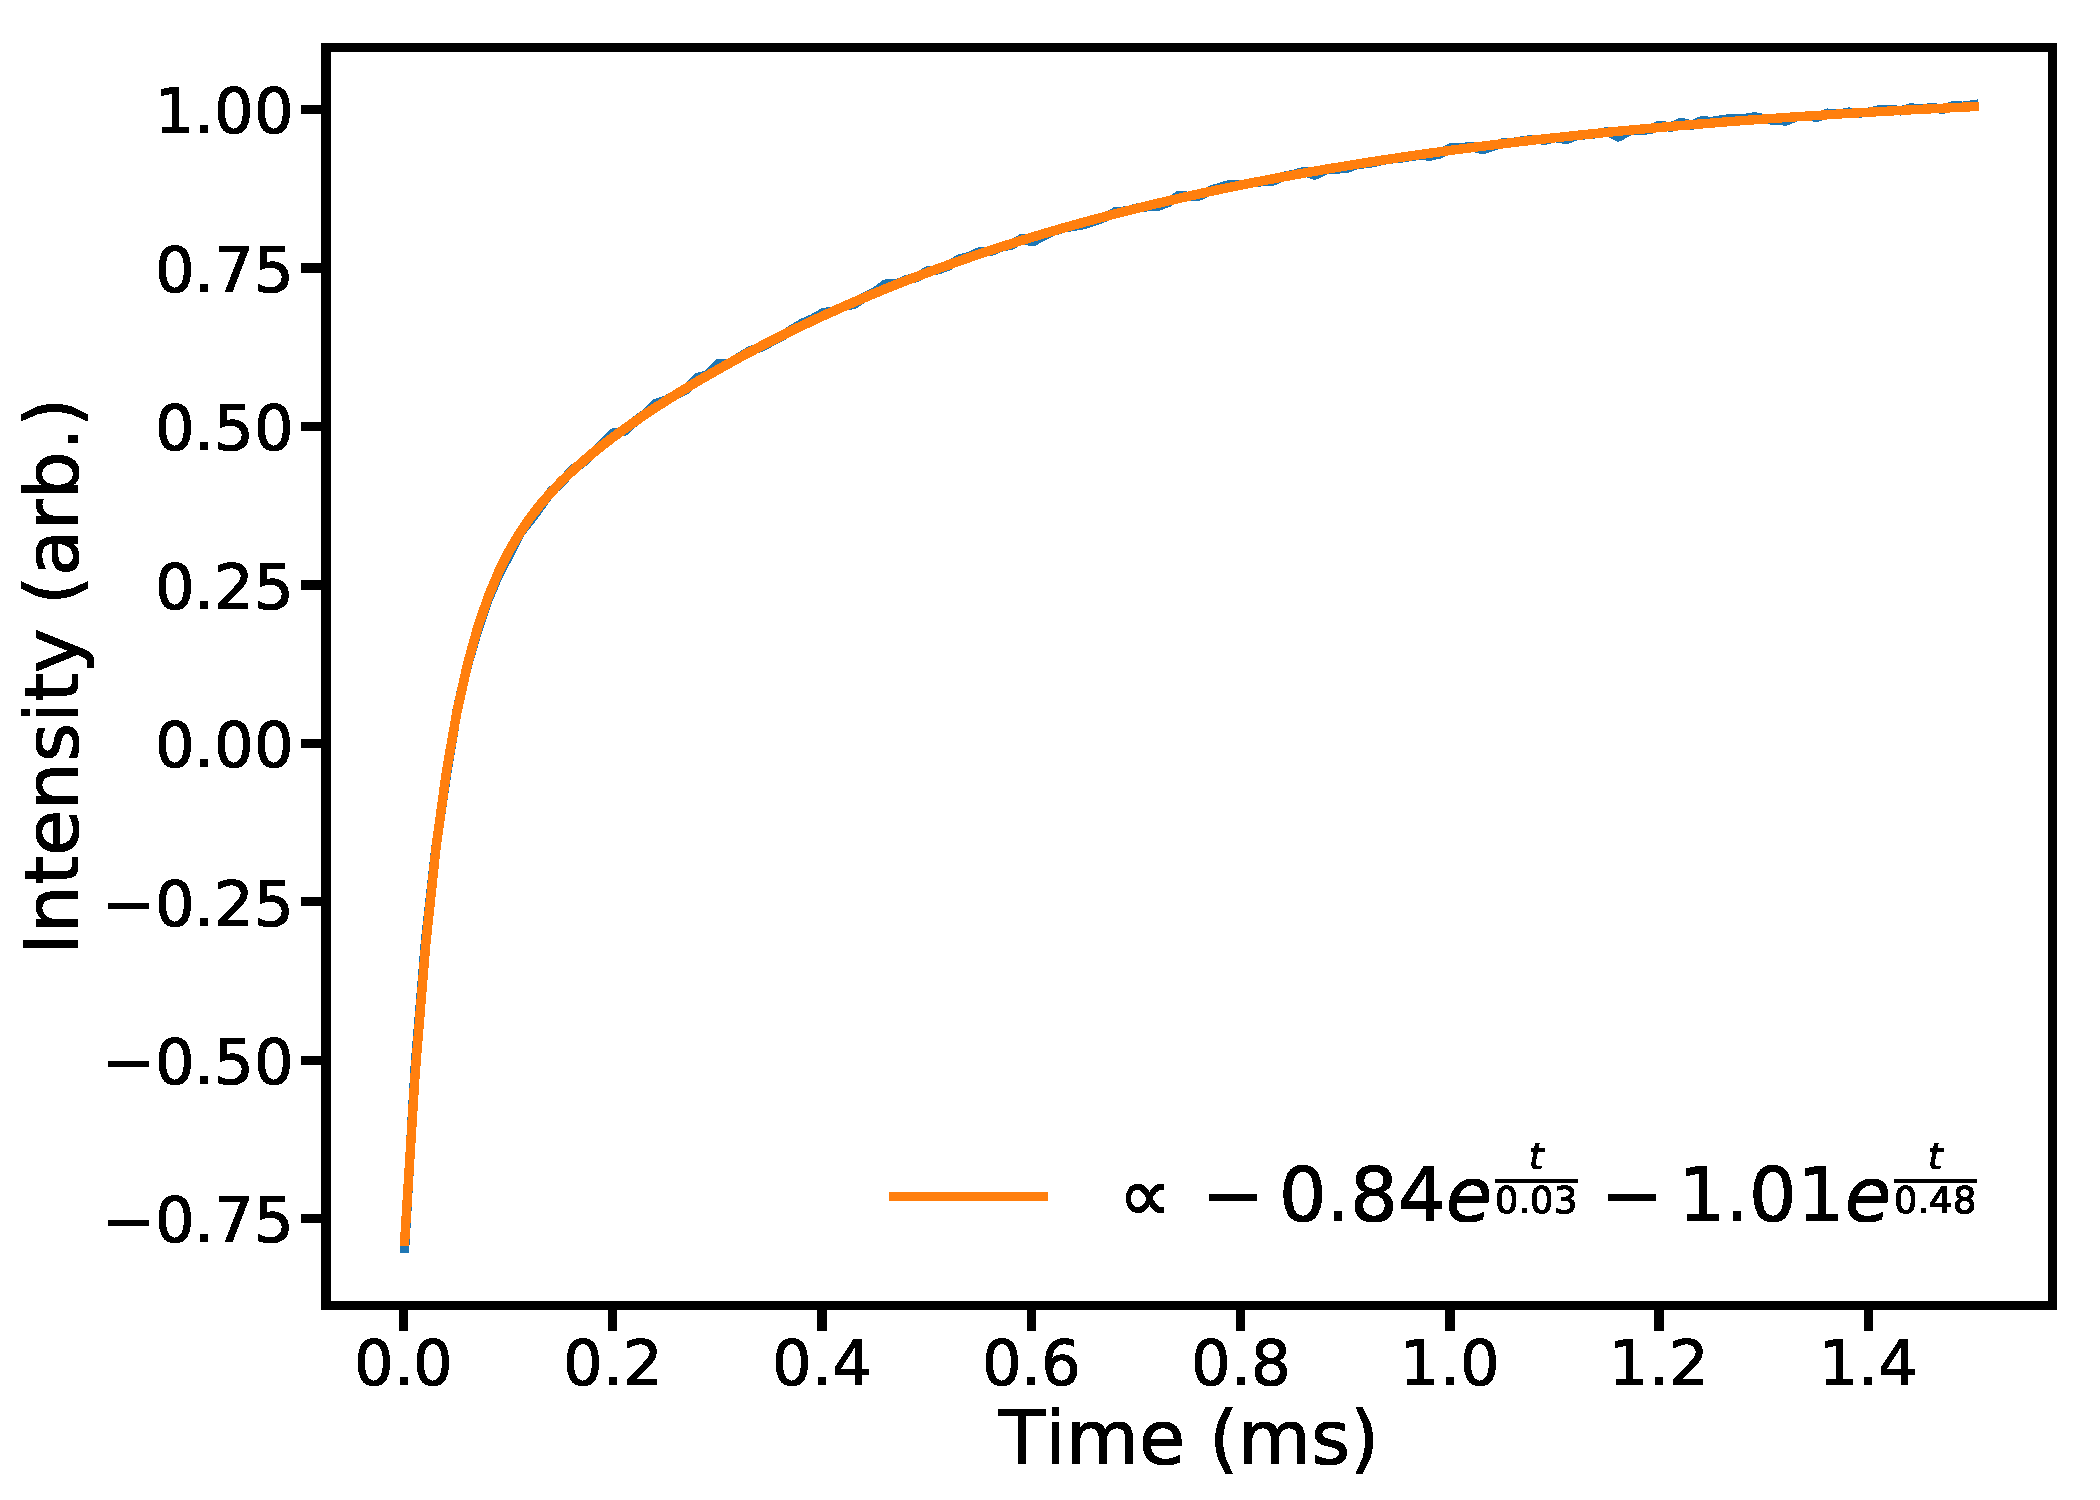
\includegraphics[width=0.8\textwidth]{Figures/T1_biExp.pdf}
\caption[Inversion recovery under laser illumination]{Inversion recovery at 8~K and under 79~mW illumination at 1070~nm. Of note is the strongly bi-exponential nature of the decay, with two distinct time constants describing it. One significantly longer than the other. A possible explanation for this is that the laser illumination is not affecting all parts of the sample. This is not unexpected as the sample is quite large, as described in section \ref{sec:lasExps}}.
\label{fig:biexpDec}
\end{figure}

Of the two time constants that describe the decay, one is significantly longer than the other and at low powers is close to the $T_1$ in the dark.
This suggests that there is a distribution of the illumination effect throughout the sample, with less affected parts relaxing more slowly than others.
This becomes more obvious when comparing the two time constants over a range of powers, as seen in figure \ref{fig:T1avsT1b}.
This shows that the shorter $T_1$ has a strict inverse polynomial dependence on laser power, whilst the longer $T_1$ cannot be similarly fit as it appears to saturate at lower powers.
Given this, it seems prudent when trying to determine the relationship between the incident light parameters and relaxation behaviour to use the shorter of the two time constants where a bi-exponential fit has been applied.
In the case of a set of data qubits close to the silicon surface, as is suggested in \cite{OGorman2014}, these qubits would be exposed to illumination and not shielded as appears to be the case for donors experiencing the long $T_1$.



\begin{figure}
\centering
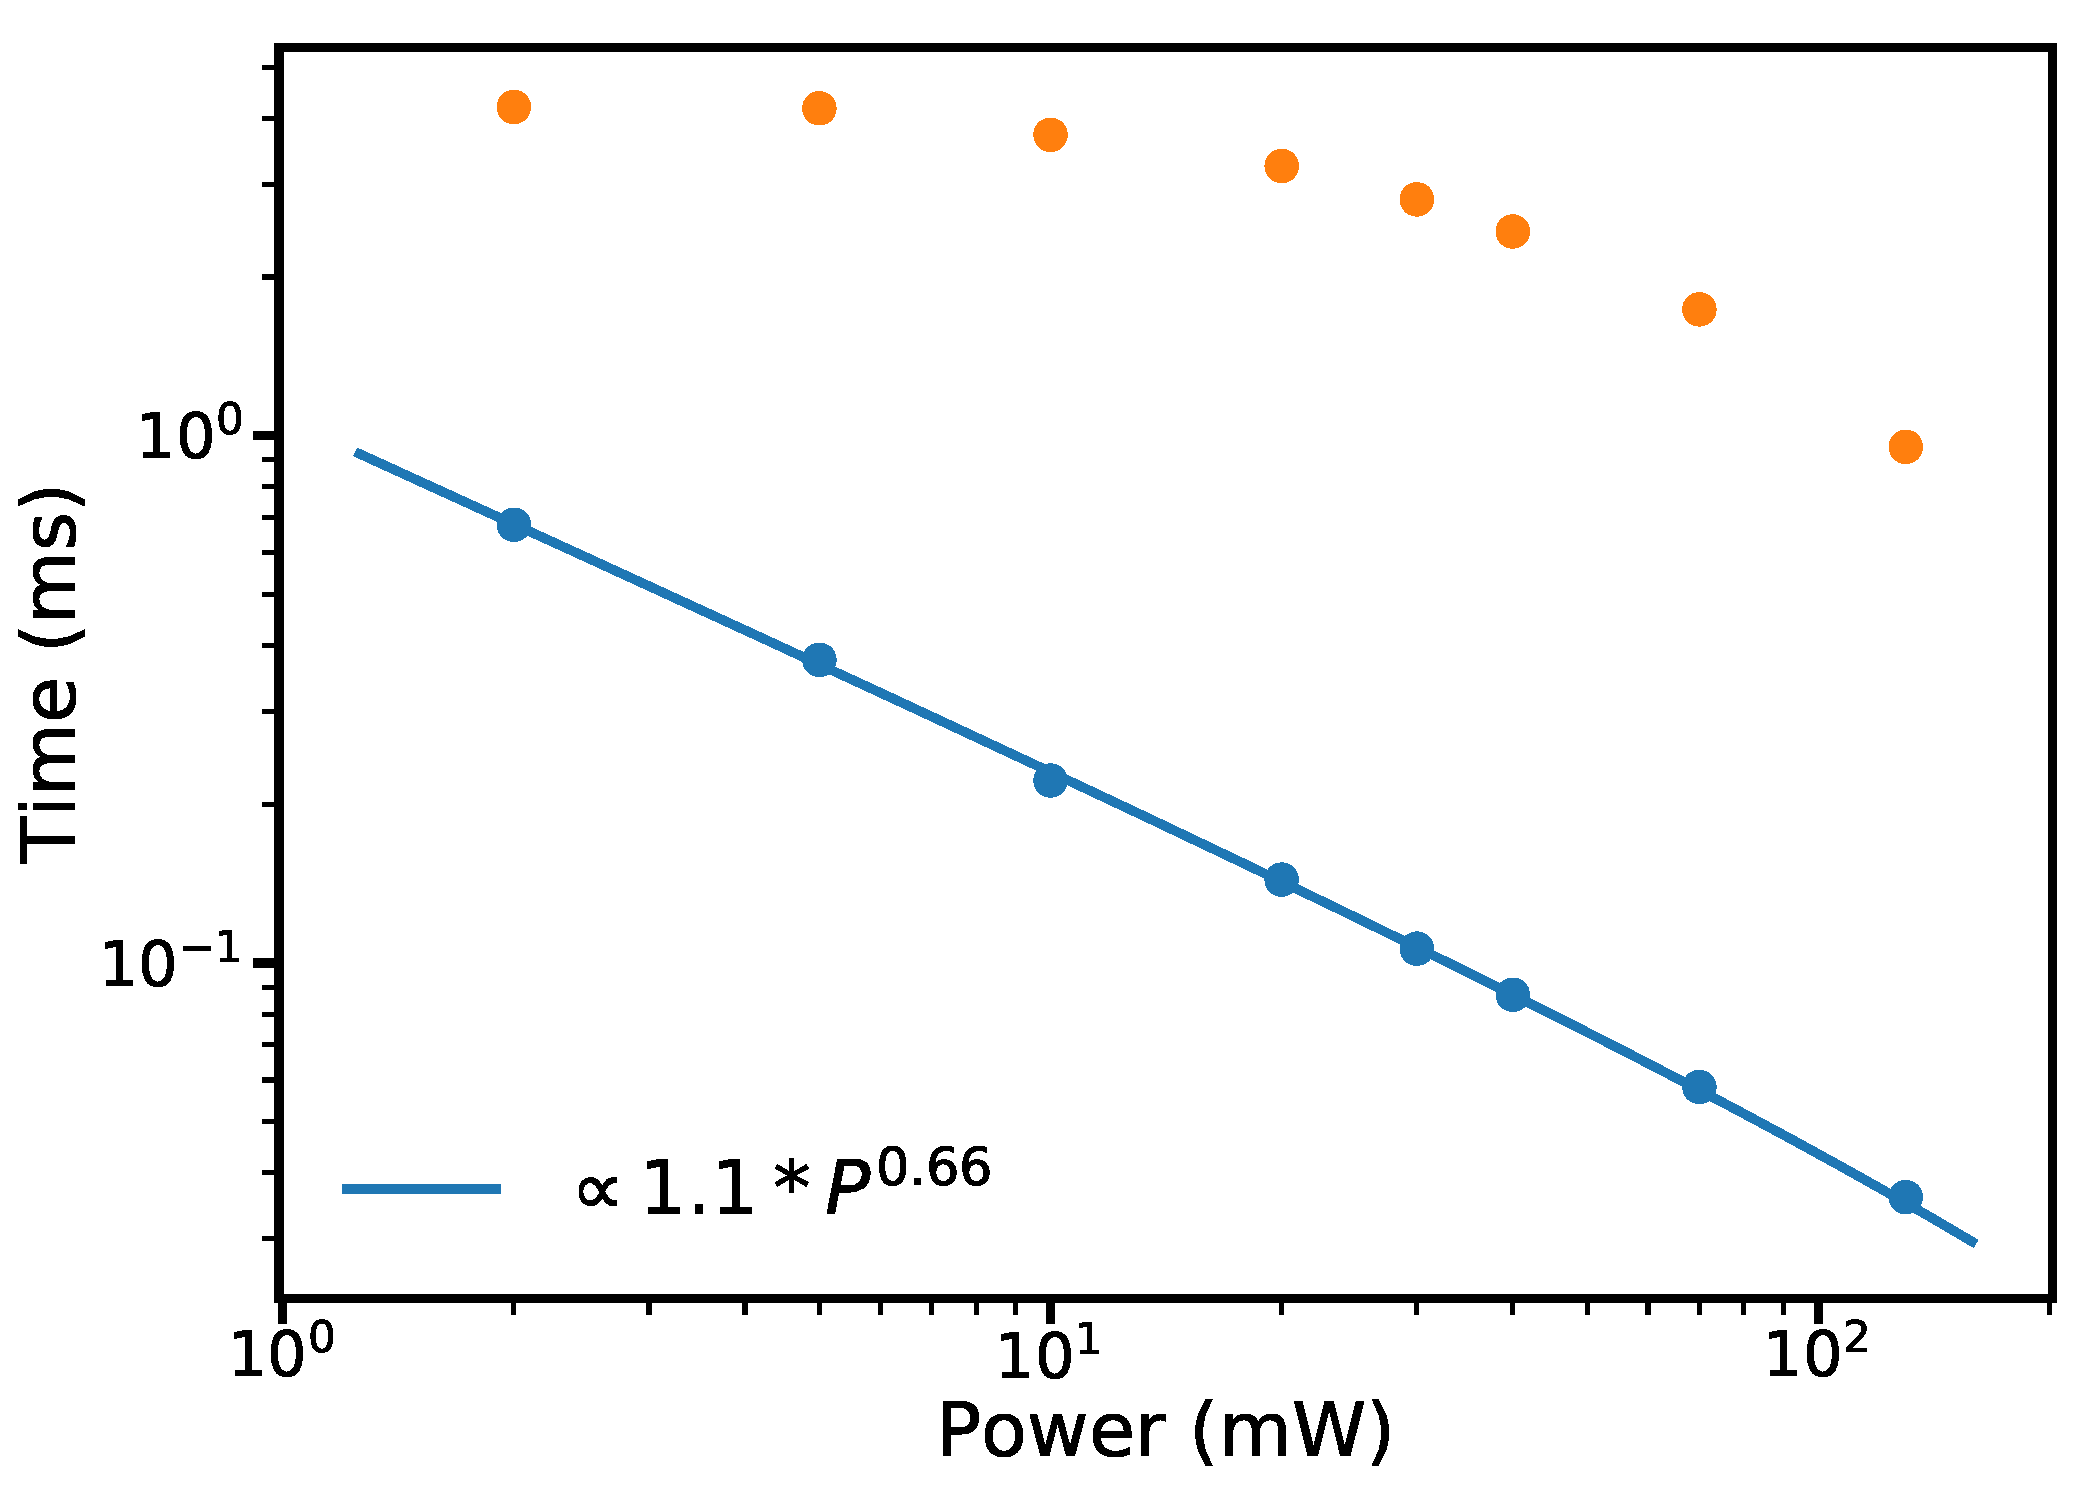
\includegraphics[width = 0.8\columnwidth]{Figures/hpT1avsT1b.pdf}
\caption[Bi-exponential relaxation decay constants]{Figure shows the two time constants for bi-exponential relaxation decay whilst under laser illumination at 1070~nm and at 8k. The shorter $T_1$ constant is well fit with a $\frac{1}{P^{0.66}}$ line. A similar fit cannot be applied to the longer $T_1$ constant, which appears to demonstrate saturation behaviour at the lower illumination powers.}
\label{fig:T1avsT1b}
\end{figure}

\subsection{High Power Wavelength Comparison}
\subsubsection{Effect on $T_1$}

Measurements comparing behaviour of $T_1$, $T_2$ and dynamical decoupling $T_2$ were performed at 3 wavelengths: 1058~nm, 1070~nm, and 1080~nm.
The shortest of these represents photon energies at approximately the band gap energy of silicon.
As such, it would be expected that this wavelength would have a stronger effect than the other two as the free carrier generation rate would be significantly higher.
This factor has previously been postulated as the dominant process affecting relaxation rates of donor electrons.
Figure \ref{fig:wavcomparison} shows the relationship between relaxation time and laser power for three wavelengths, fitted according to $A/t^{\alpha}$.
This fit is applied due to the expected relationship between power and photon density at the sample being approximately $\frac{1}{x}$.
The observation that the relationship between power and $T_1$ time is close to linear on a log-log graph also suggests that it is based upon a power law.
The power for each wavelength is $0.73\pm.002, 0.68\pm.0002$ and $0.68\pm.003$, in order of increasing wavelength.
Measurements were also taken at 2~mW and 5~mW but are not included here as the large error in the power values makes them unsuitable for comparison between data sets.
What is clear from the above graph is that there is an observable difference between the case of 1058~nm illumination and the two higher wavelengths.
This is to be expected given that 1058~nm is at approximately the silicon band gap, meaning that absorption of photons will be higher and free carrier generation significantly higher than with less energetic photons.
Although the higher wavelengths have a lesser effect, there is still a strong reduction in relaxation times.
The similarity between the effects suggest that the mechanisms responsible for the increased rate do not have a strong dependence on individual photon energy once the band-gap is passed, instead the power of the incident illumination is dominant.

\begin{figure}
\centering
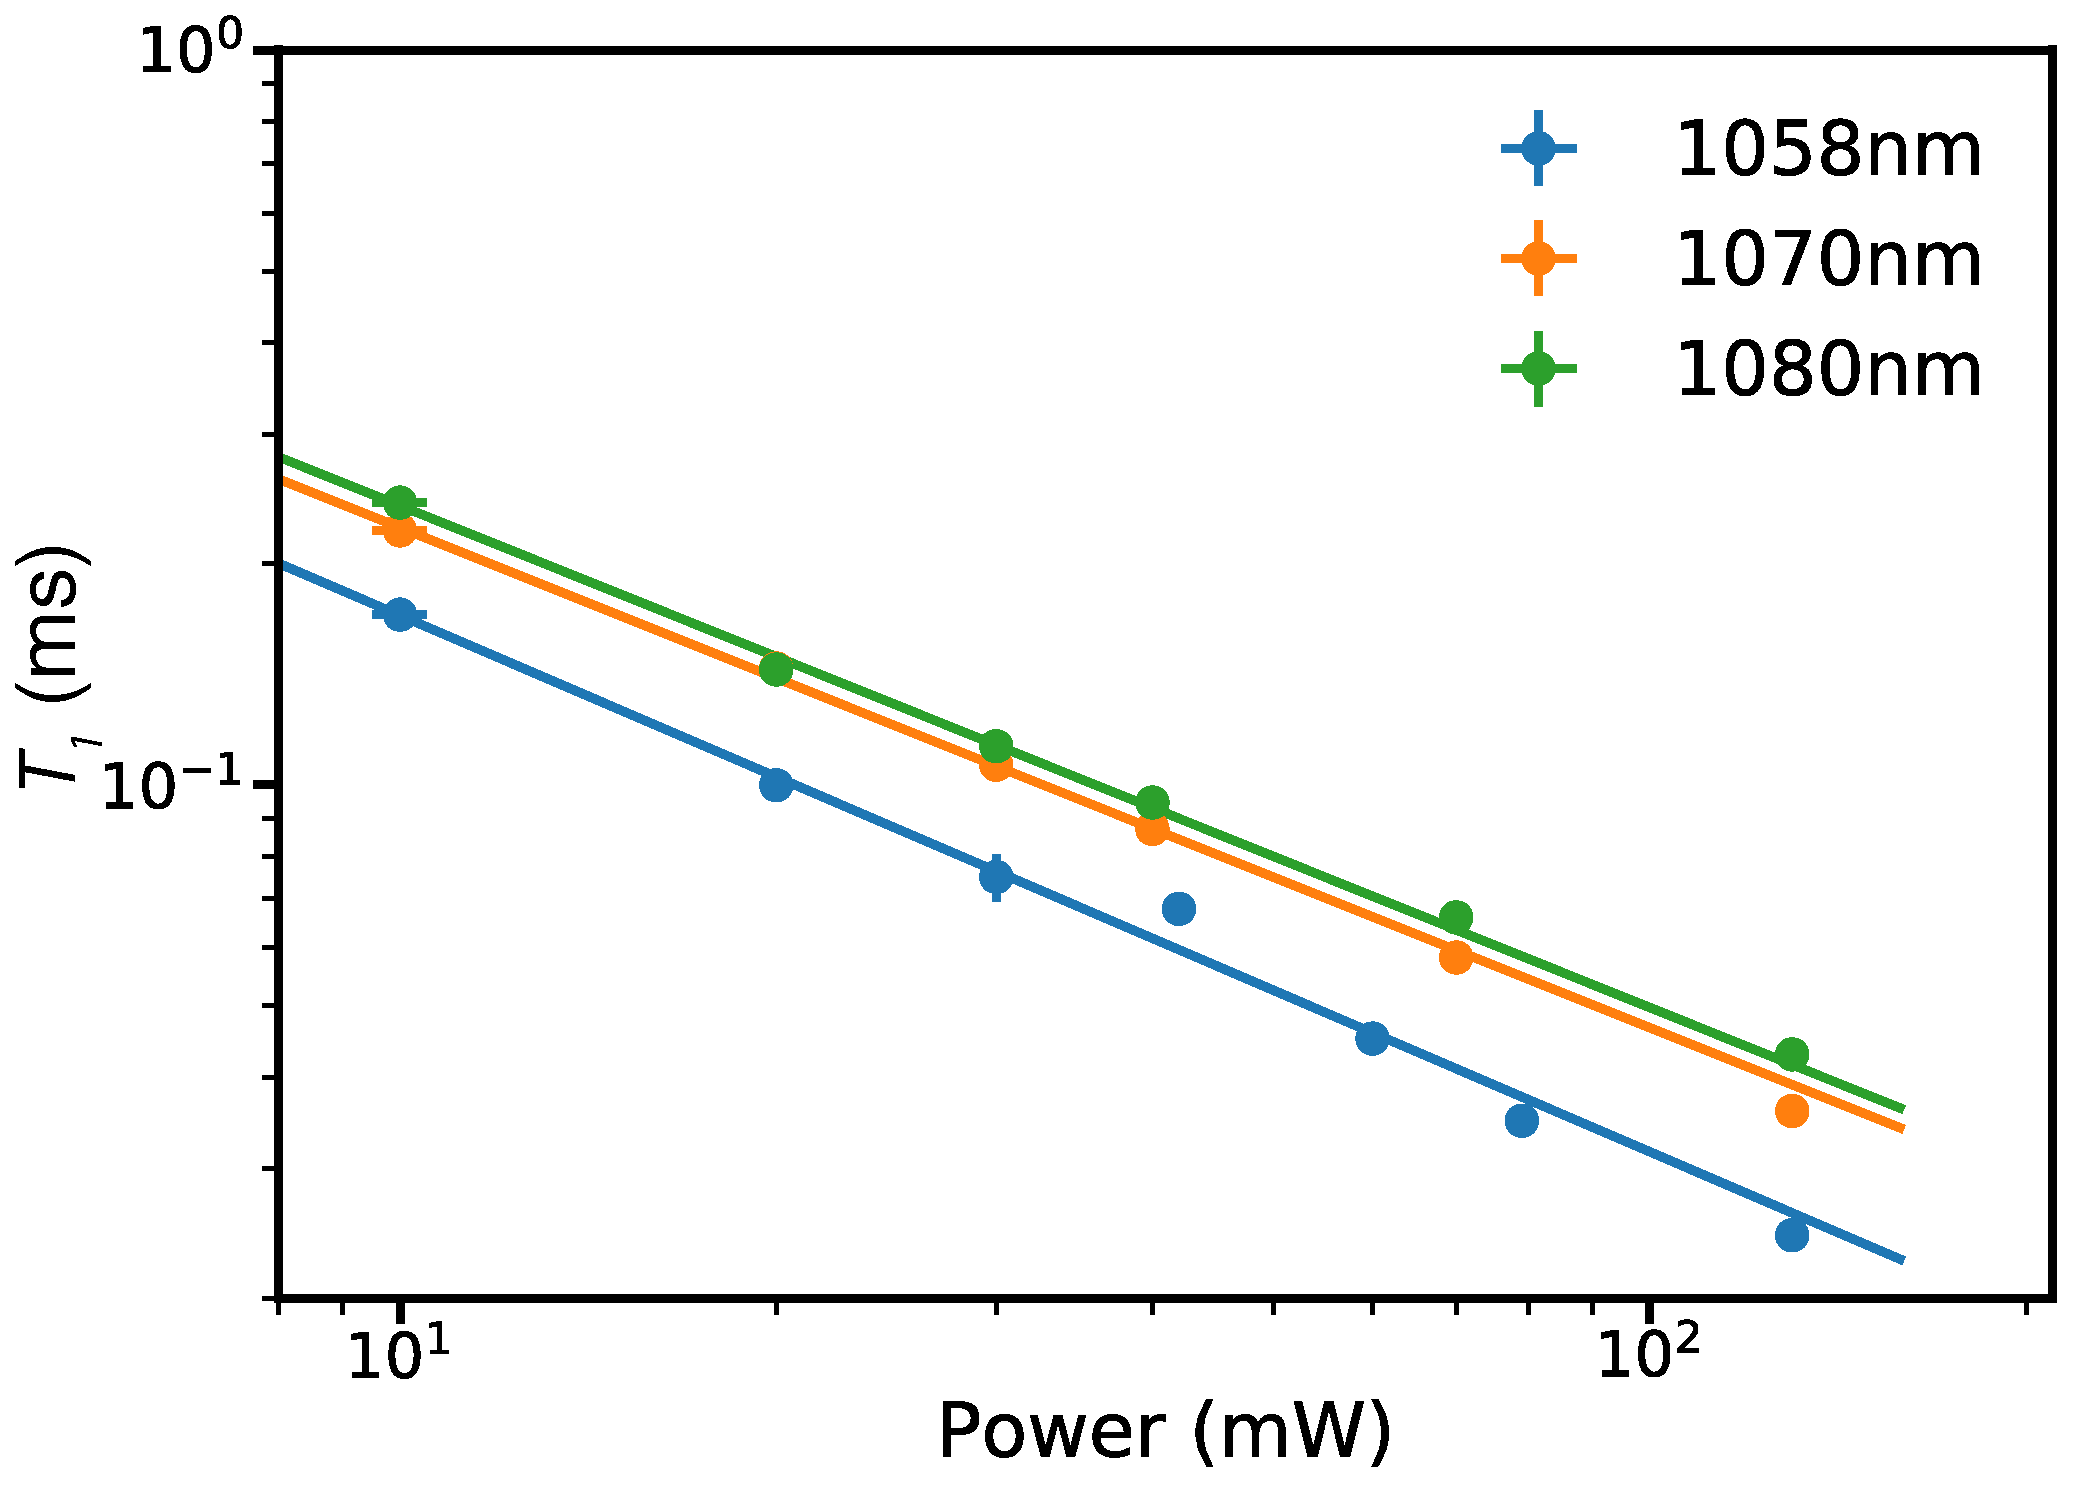
\includegraphics[width = 0.8\columnwidth]{Figures/Logwavelengthcomp.pdf}
\caption[Relaxation comparison at 8~K and 1058~nm, 1070~nm, and 1080~nm illumination]{Figure shows the relationship between laser power and relaxation time for 3 different wavelengths: 1058~nm, 1070~nm and 1080~nm.}
\label{fig:wavcomparison}
\end{figure}

The impact of illumination on relaxation rates observed here is in line with predictions.
Increased wavelength results in a slower relaxation rate at equivalent powers, with a more significant change being observed as the silicon band gap energy is crossed.
Relaxation rates follow a $a/P^{\alpha}$ curve.

\subsubsection{Effect on $T_2$}

Whilst the $T_1$ time is important for quantum information processing, as it ultimately limits computation time, $T_2$ is in most cases the limiting factor in qubit coherence.
The mechanisms that limit $T_2$ in spins were discussed in section \ref{sec:litdecoherence}.
Of particular worry is that a significant number of free electrons in the silicon conduction band could create time dependent magnetic fields at the observed donor spins.
If this is the case then there could be an impact on the $T_2$ time beyond the effect of reduced $T_1$.
Figure \ref{fig:t1vst2wav} shows how $T_1$ and $T_2$ vary with laser power for 1058~nm and 1070~nm.
What is clear in both cases is that there does not appear to be a significant effect beyond $T_2$ being limited by $T_1$.
In both graphs it is clear at the lower powers that $T_2$ is beginning to saturate to the value in the dark of $220\mu$s.
The fact that there is no clear difference between the effects in the 1058~nm case and the 1070~nm case is interesting.
It suggests that, although there is clearly a greater magnitude of effect in the lower wavelength case, if the mechanism is different then it has no impact on $T_2$ above and beyond the extra $T_1$ limitation.


\begin{figure}
\centering
\begin{subfigure}[b]{0.5\columnwidth}
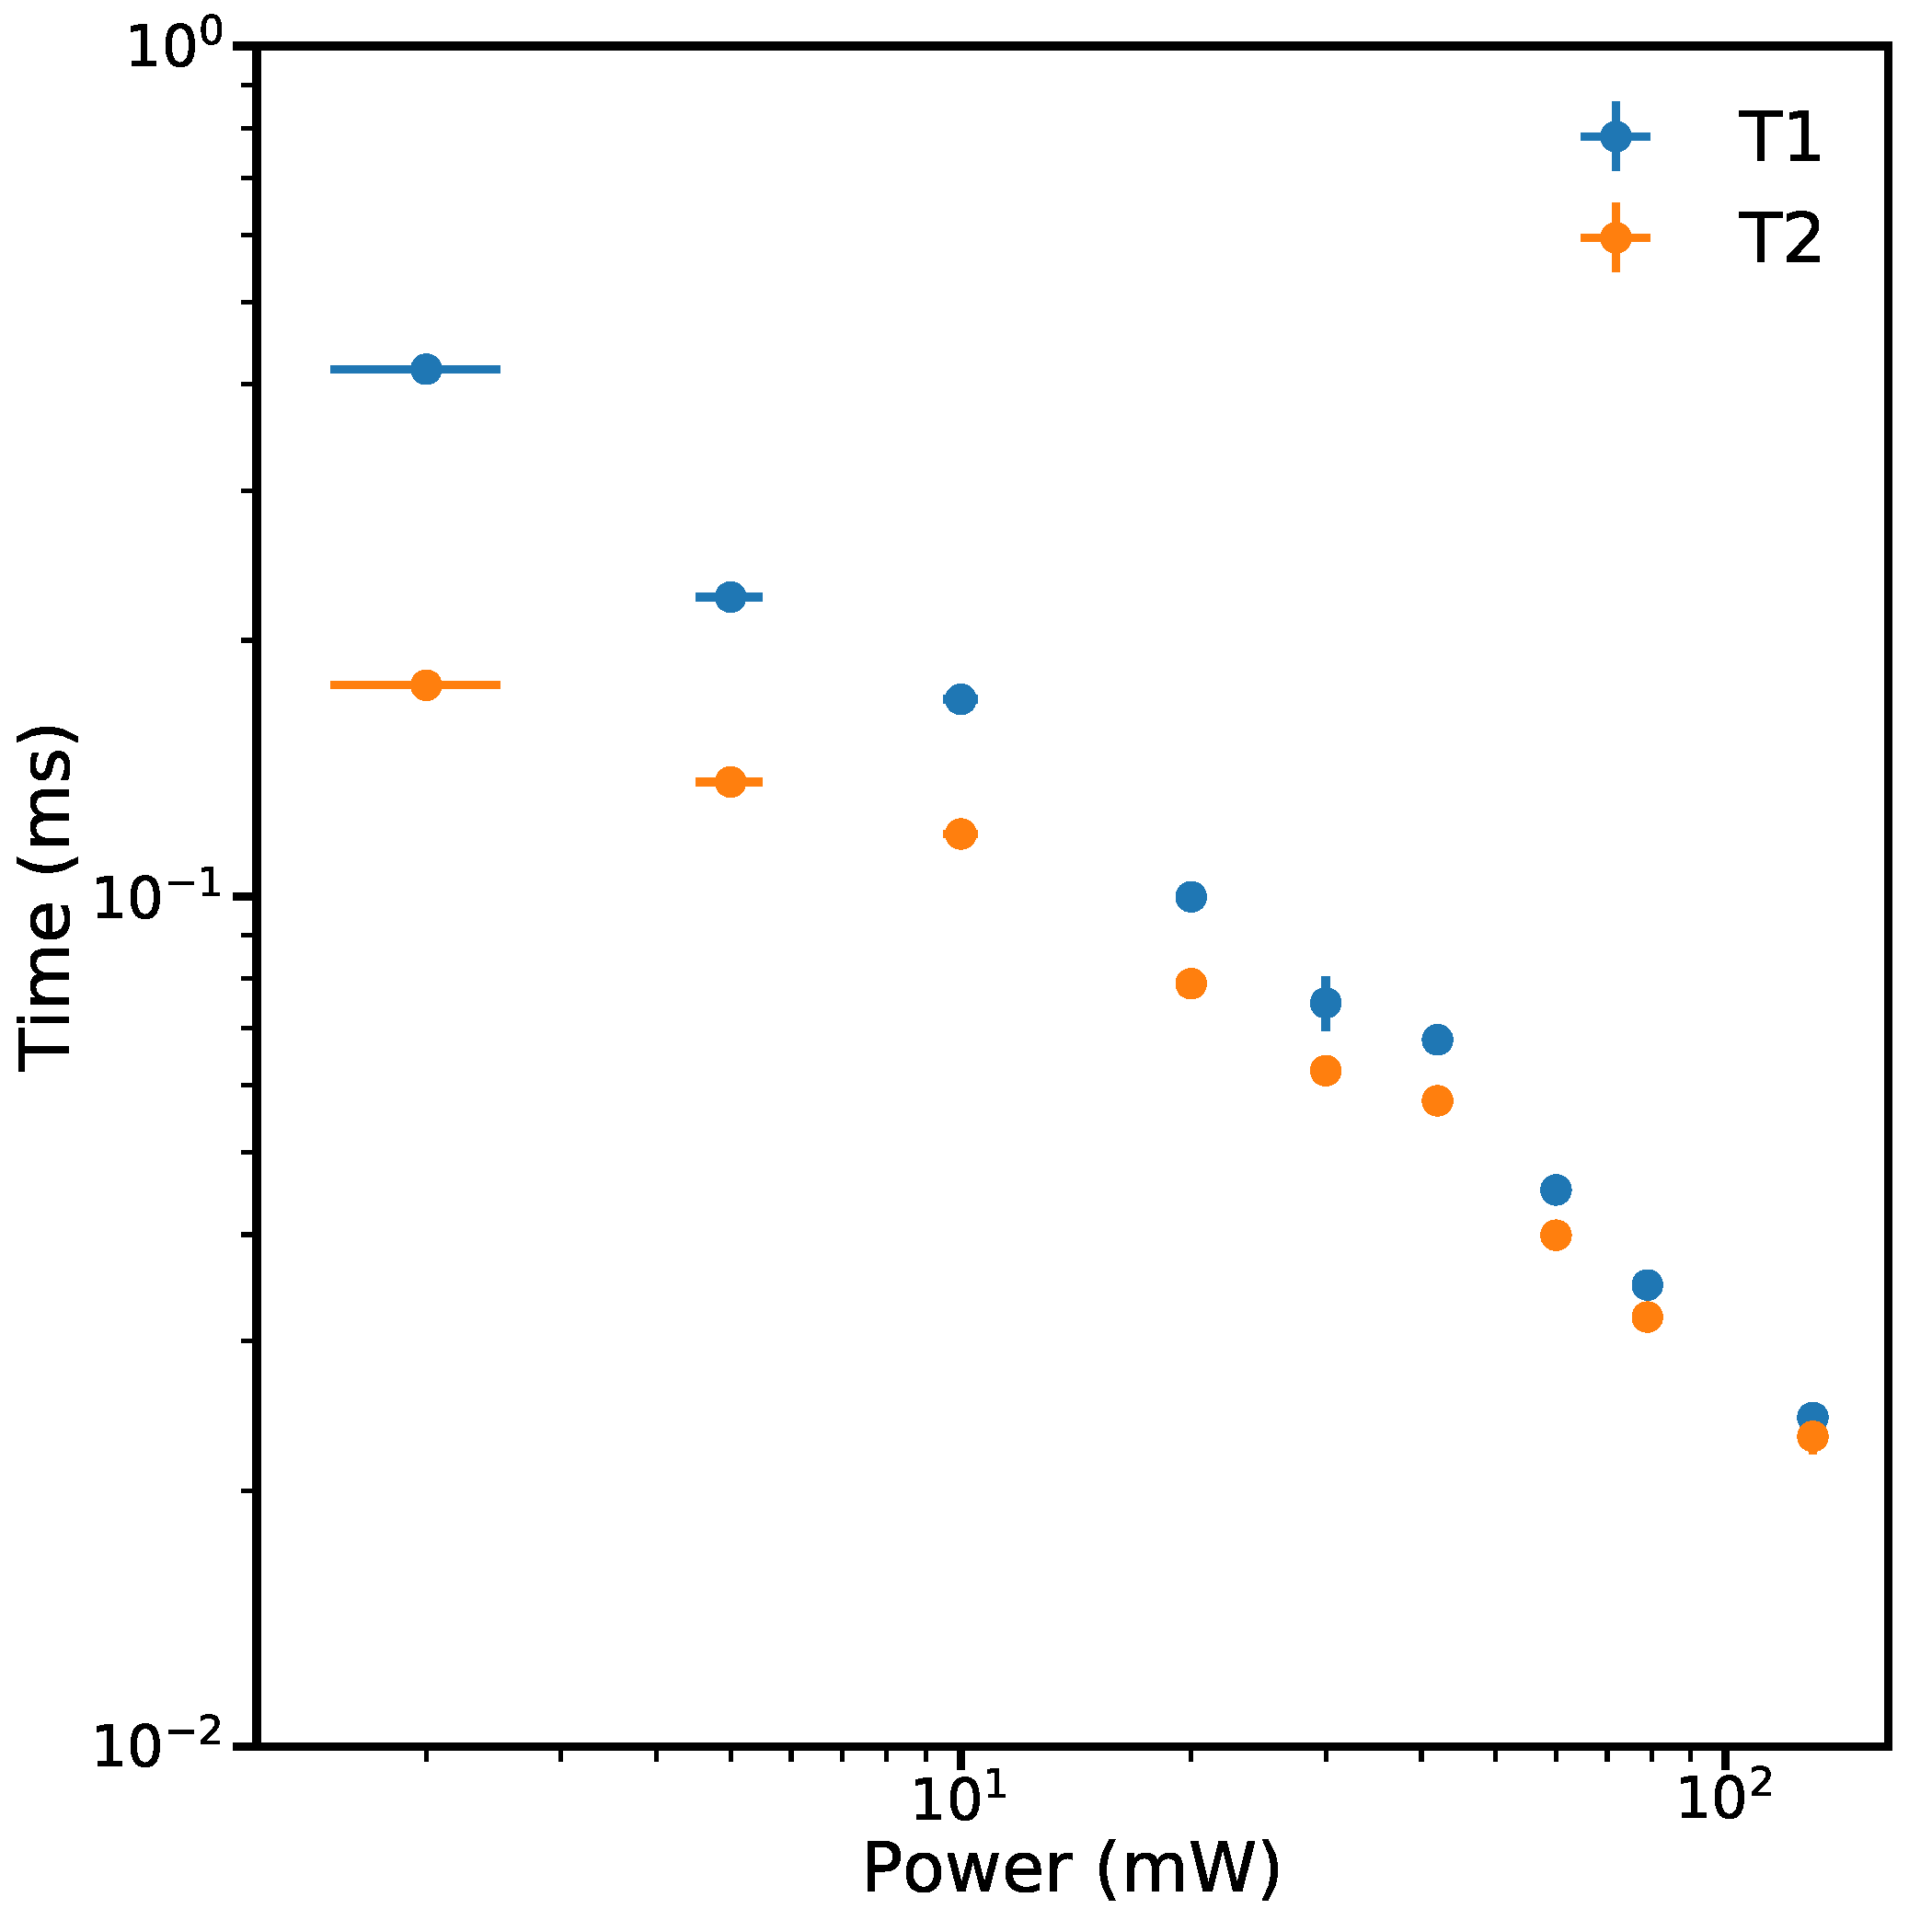
\includegraphics[width = \columnwidth]{Figures/8kT1vsT21058.pdf}{(a)}
\end{subfigure}%
\begin{subfigure}[b]{0.5\columnwidth}
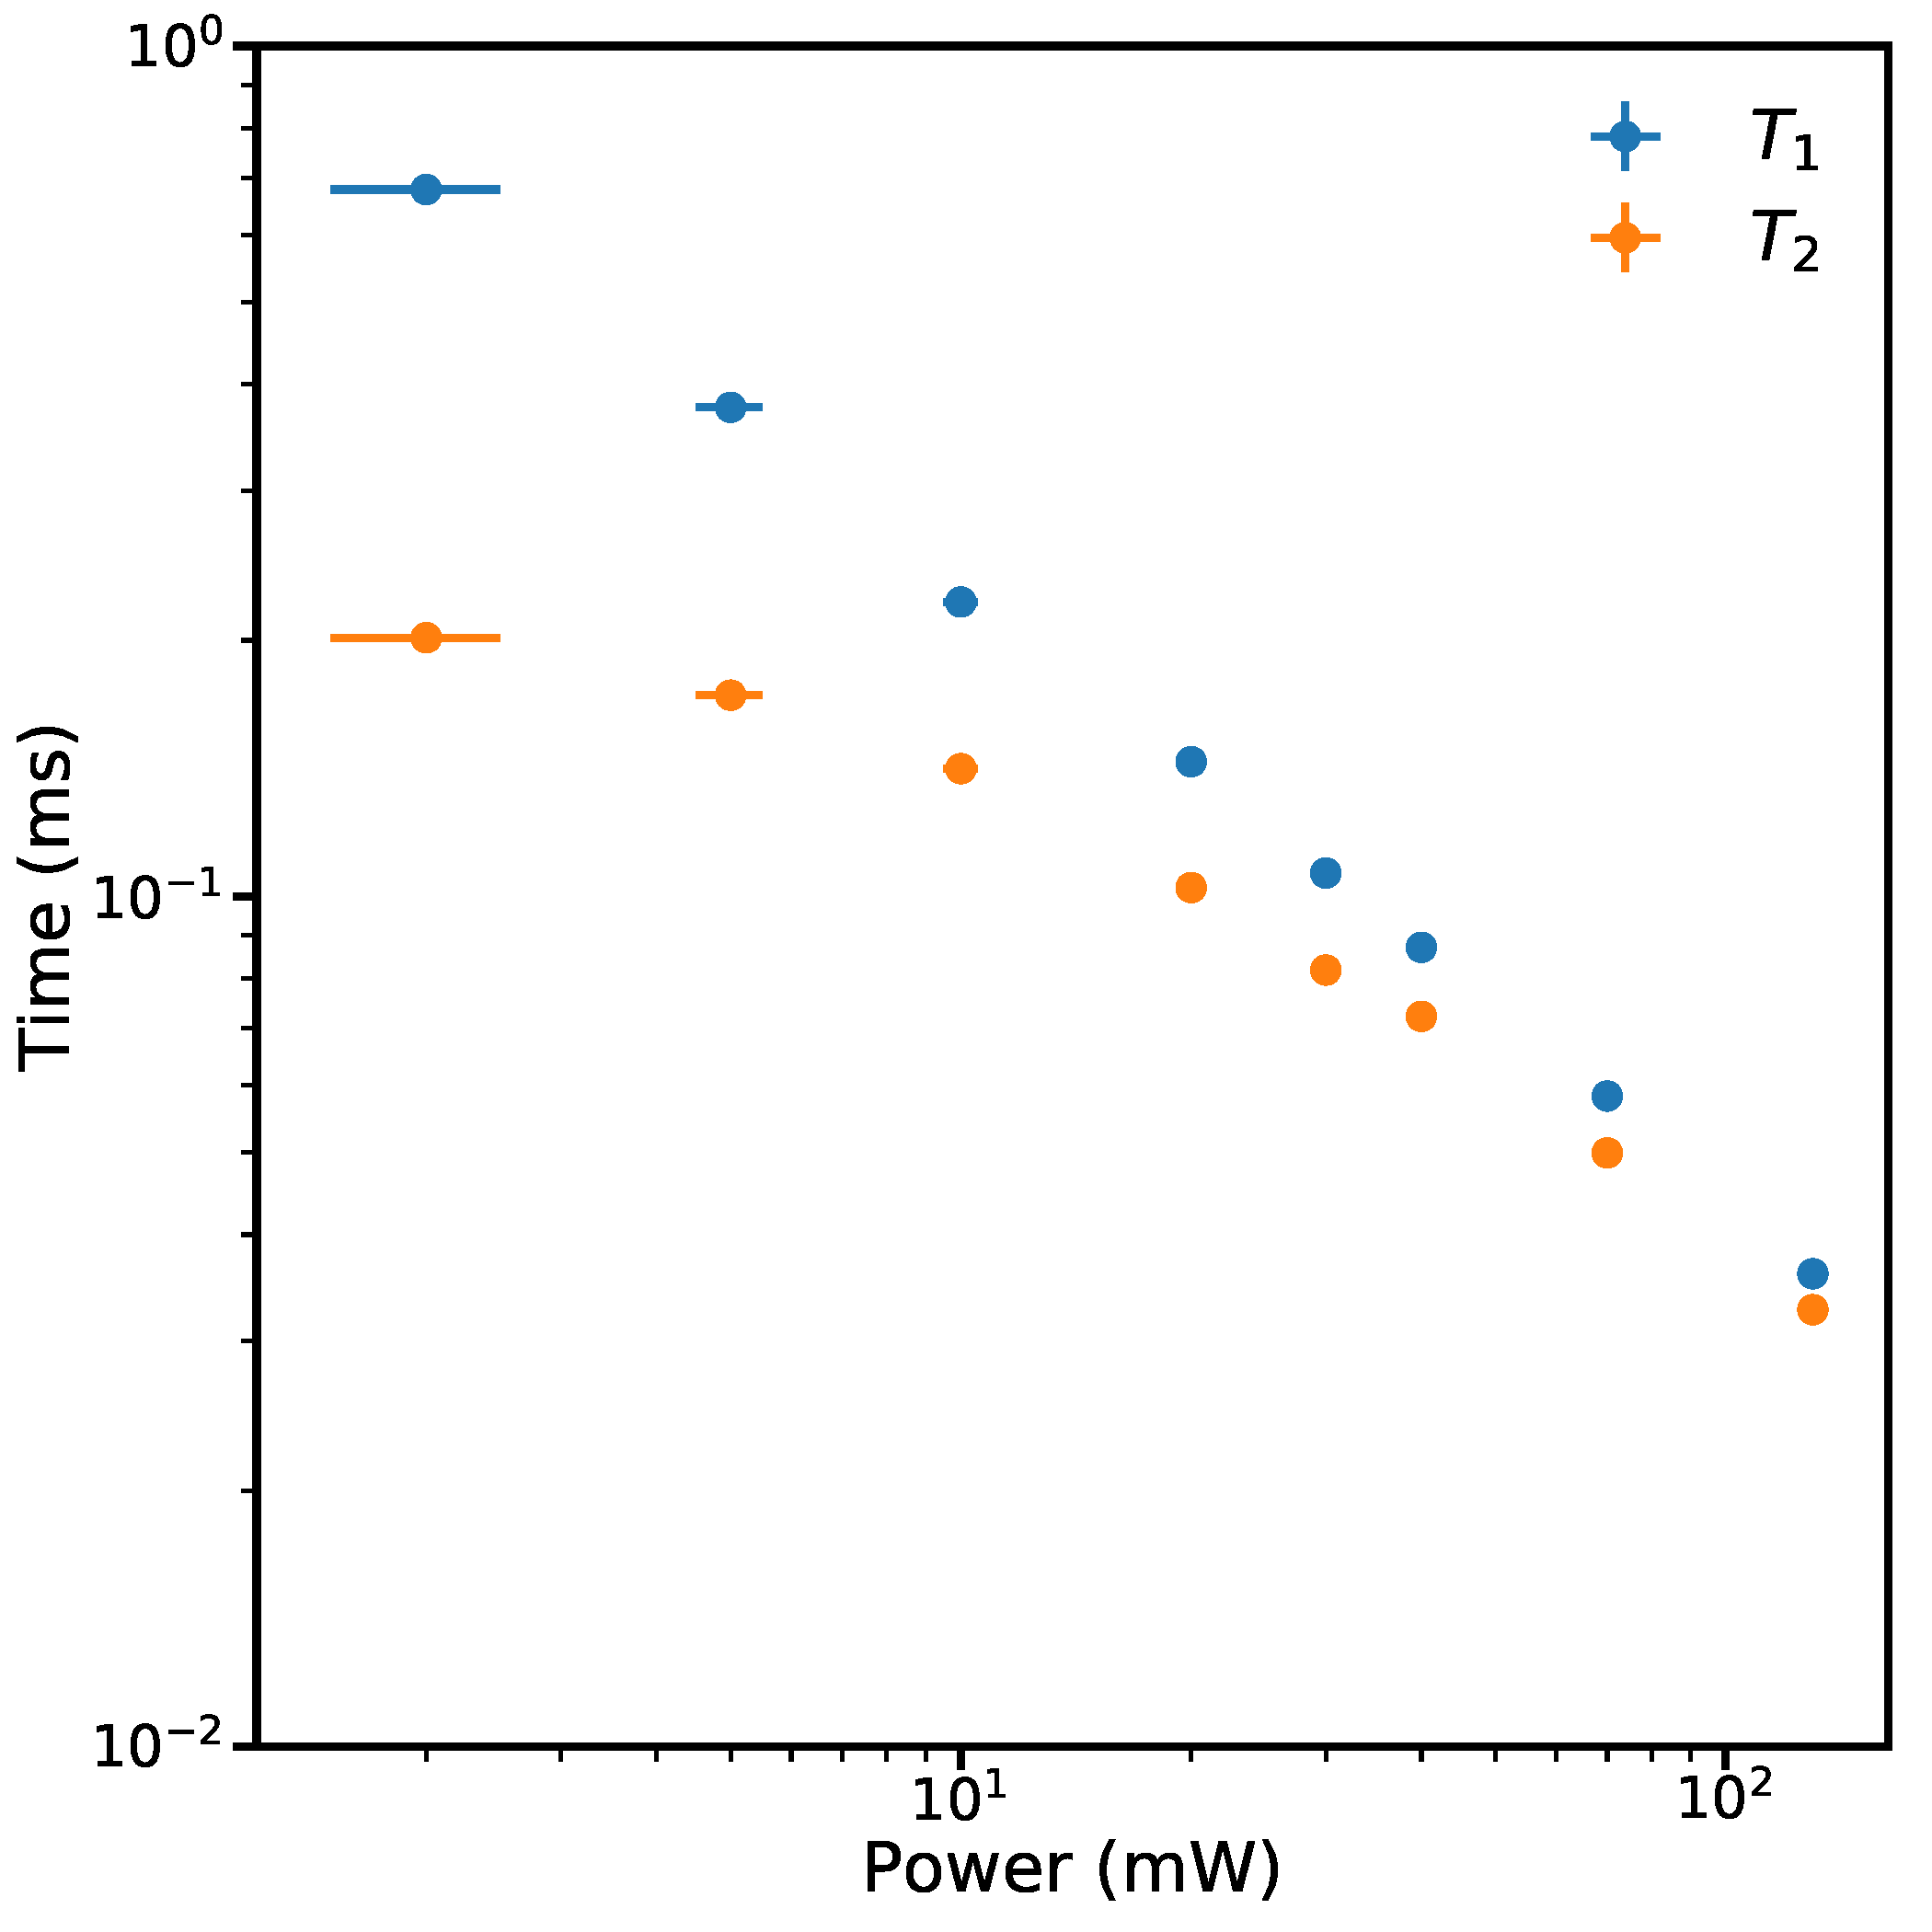
\includegraphics[width=\columnwidth]{Figures/T1vsT11070.pdf}
\end{subfigure}%
\caption[$T_1$ vs $T_2$ for 1058~nm and 1070~nm]{Figures showing how both $T_1$ and $T_2$ vary with laser power, presented on the same scale for ease of comparison. At high powers $T_1$ is observed to be close to $T_2$, essentially limiting it. }
\label{fig:t1vst2wav}
\end{figure}

\begin{figure}
\centering
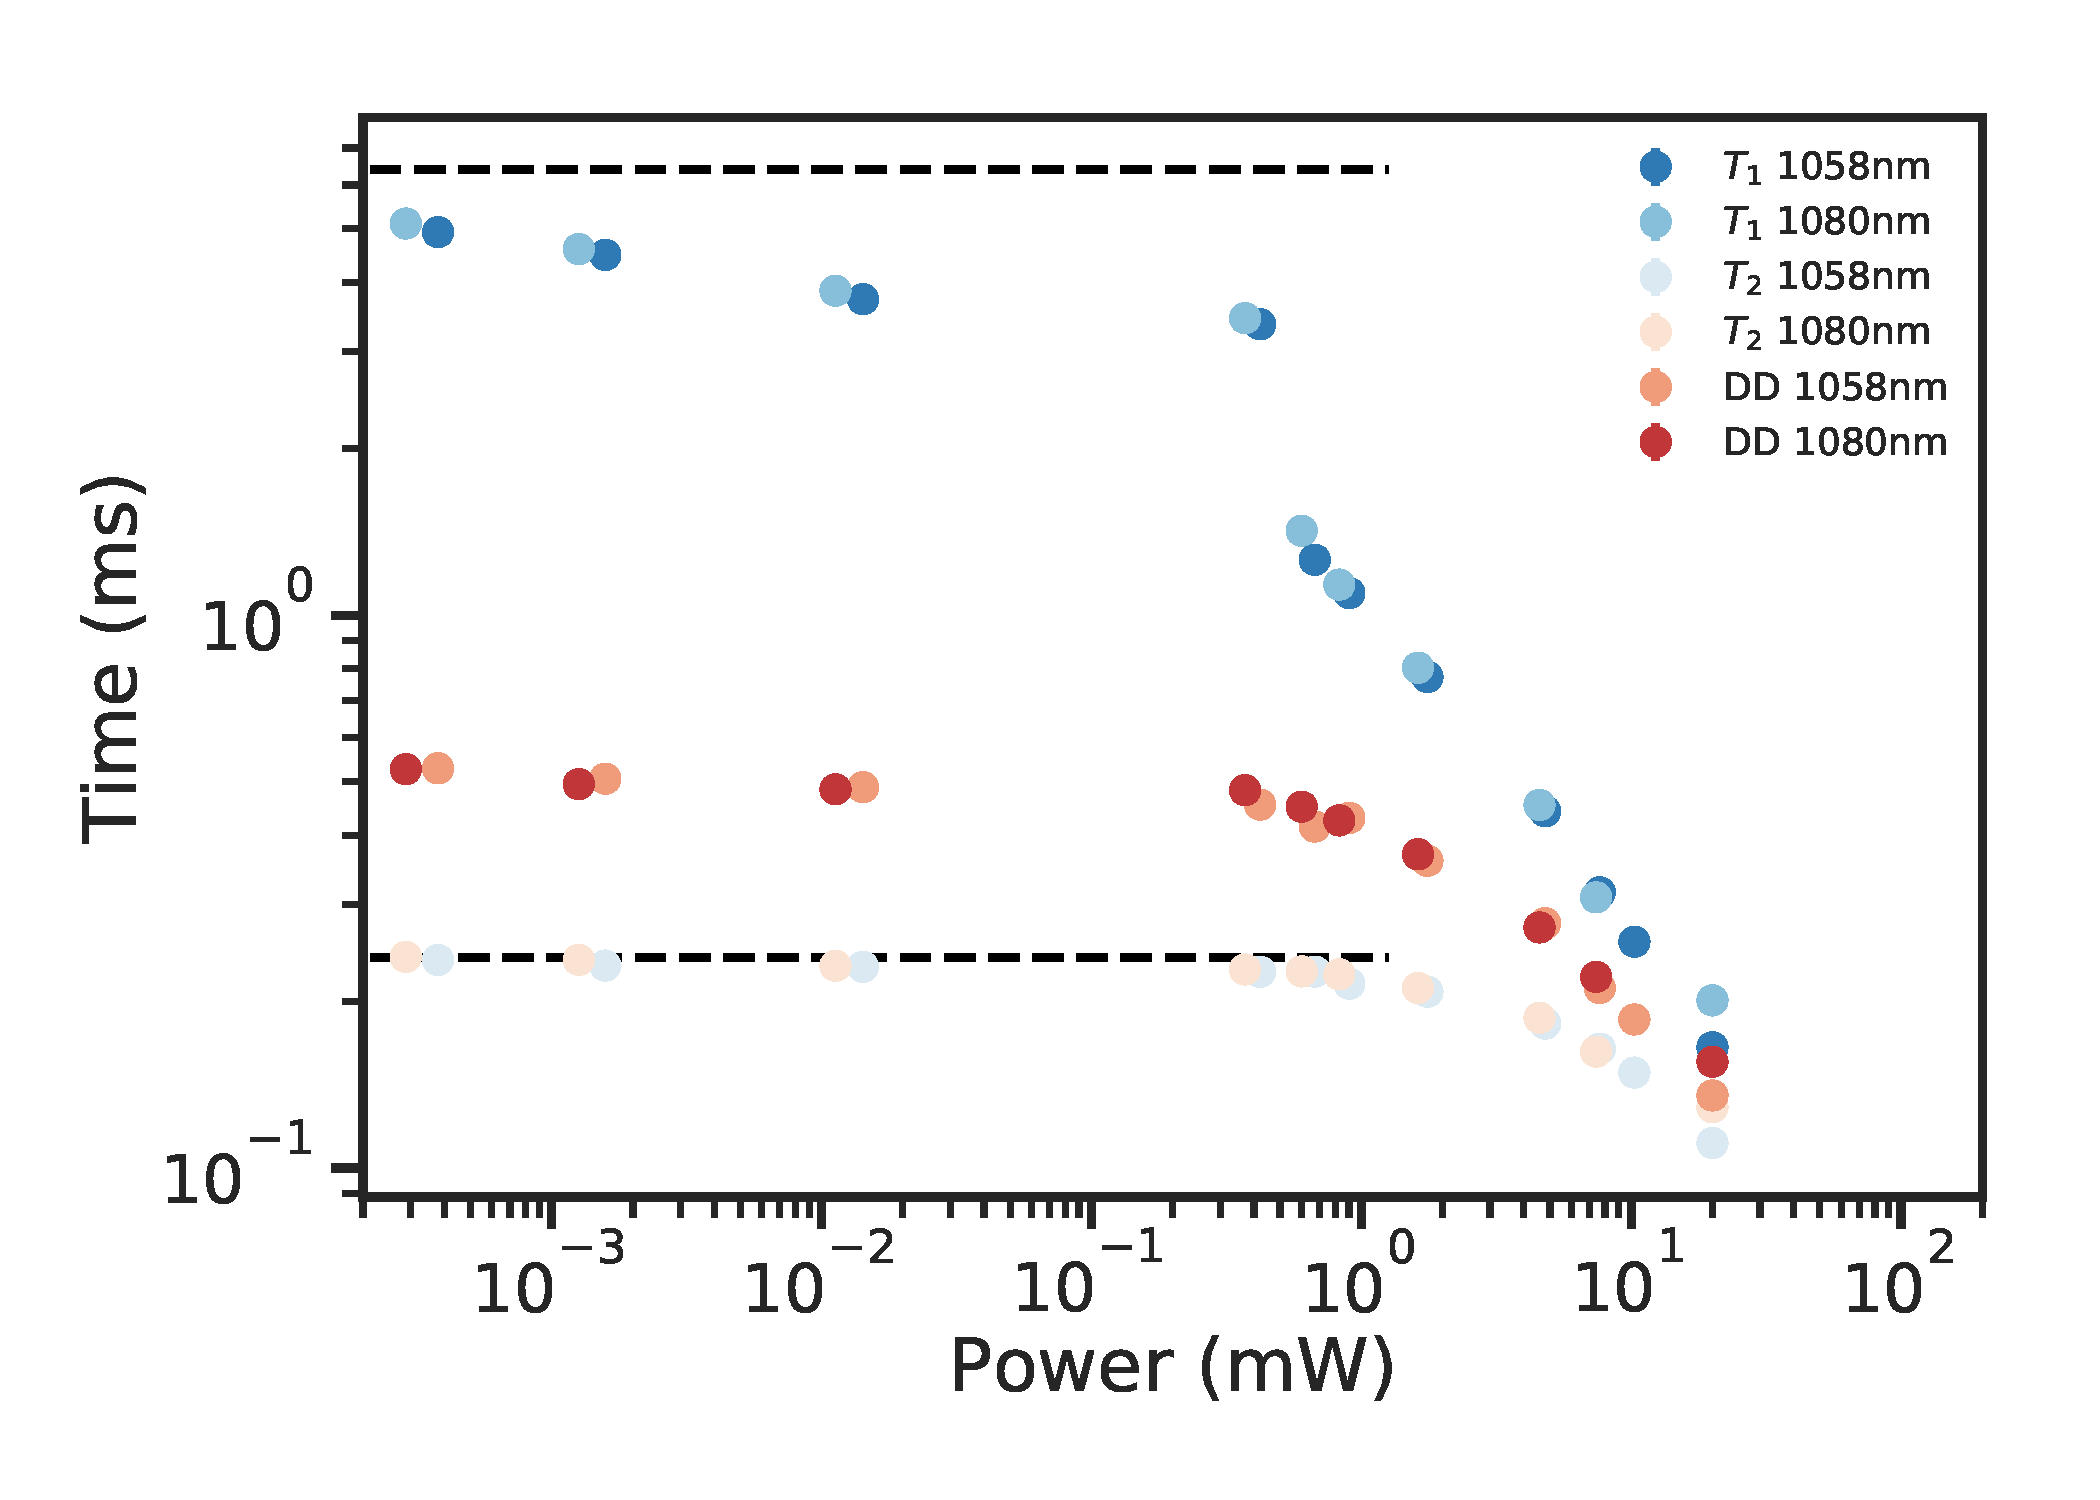
\includegraphics[width=0.8\columnwidth]{Figures/T1vsT2vsDD1058and1080.pdf}
\caption[Low power $T_1$ and $T_2$ comparison]{Figure shows the impact of laser illumination at low power and at wavelengths of 1058~nm and 1080~nm. For reference $T_1$ and $T_2$ in the dark are shown as black dotted lines ($T_1$ is the longer time-scale). $T_1$ is observed to saturate at very low laser powers, as it becomes close to the $T_1$ in the dark. Included is the coherence time for a 4 $\pi$ pulse dynamical decoupling sequence. This shows the expected increase in decoherence time at lower powers and continues to have an advantage over a traditional Hahn echo sequence as both begin to be reduced. Small differences in power at equivalent data points are due to the transmission of ND filters varying slightly with wavelength.}
\label{fig:t1vst2lowpow}
\end{figure}
The next question to be answered is whether the $T_1$ time will demonstrate a similar saturation behaviour as laser power is reduced as is demonstrated by $T_2$.
To see this lower powers must be used, achieved as described in section \ref{sec:lasExps} through the use of ND filters.
The results are shown in figure \ref{fig:t1vst2lowpow}.
These demonstrate that the $T_1$ does indeed saturate towards the dark $T_1$ at very low powers.
Of interest is the behaviour of the $T_2$ time as the $T_1$ time starts to be reduced significantly.
The $T_2$ time clearly starts to decrease \textit{before} it is strictly limited by $T_1$.
Several factors could explain this.
The first possibility is that the creation of free carriers promoted from the valence band is causing extra magnetic field noise at donor sites, reducing their $T_2$ time.
The difficulty with this particular mechanism is that there appears to be very little difference, at these low powers, between the $T_2$ times at the different wavelengths.
Were this to be a significant effect then one would anticipate that it would be noticeably stronger in the lower wavelength case.
The alternative factors are $T_1$ related, were discussed in section \ref{sec:mechrelax}, and account well for the observed behaviour.
As relaxation rate increases, decoherence rate is also observed to increase before being strictly limited by the relaxation rate.
This is due in the main to the additional spectral diffusion processes as a result of neighbouring donor electron spin flips.
As seen in figure \ref{fig:t1vst2lowpow}, dynamical decoupling gives an advantage over a Hahn echo sequence for decoherence time.
As this is a natural silicon sample the advantage in the dark is to be expected, a small advantage remains even when the dynamical decoupling $T_2$ is shorter than the Hahn echo.
This suggests that the 4 pulse echo sequence is providing some protection from the mechanisms causing the increased decoherence rate - likely the spectral diffusion processes associated with an increased relaxation rate.
\\
The results here allow one important conclusion - there do not seem to be significant decoherence effects caused by laser illumination beyond the impact of an increased relaxation rate.
This is an important as it demonstrates that laser based read-out of measurement qubits is possible without destroying the quantum information held in data qubits, as long as power is sufficiently low.
To explore whether the impact on relaxation rates at a given laser power can be reduced I turn now to examine results at a lower temperature - 7k.

\subsection{Temperature Comparison}

A temperature comparison is useful primarily to give insight into the mechanism of increased relaxation rate.
A first expectation is that relaxation rate will begin to saturate at lower laser powers at lower temperatures, in line with the longer dark relaxation rate.
Particularly revealing will be a direct comparison between relaxation rates at the same wavelength and power, but at different temperatures.
If these are the same then it would suggest that whatever mechanism affecting the relaxation rate is temperature independent - potentially ruling out heating as a cause.
Figure \ref{fig:t1tempcomp} shows how $T_1$ changes with laser power at 1058~nm and at 7~K and 8k, with $T_1$s in the dark of 2.77~ms and 32.2~ms respectively.

\begin{figure}
\centering
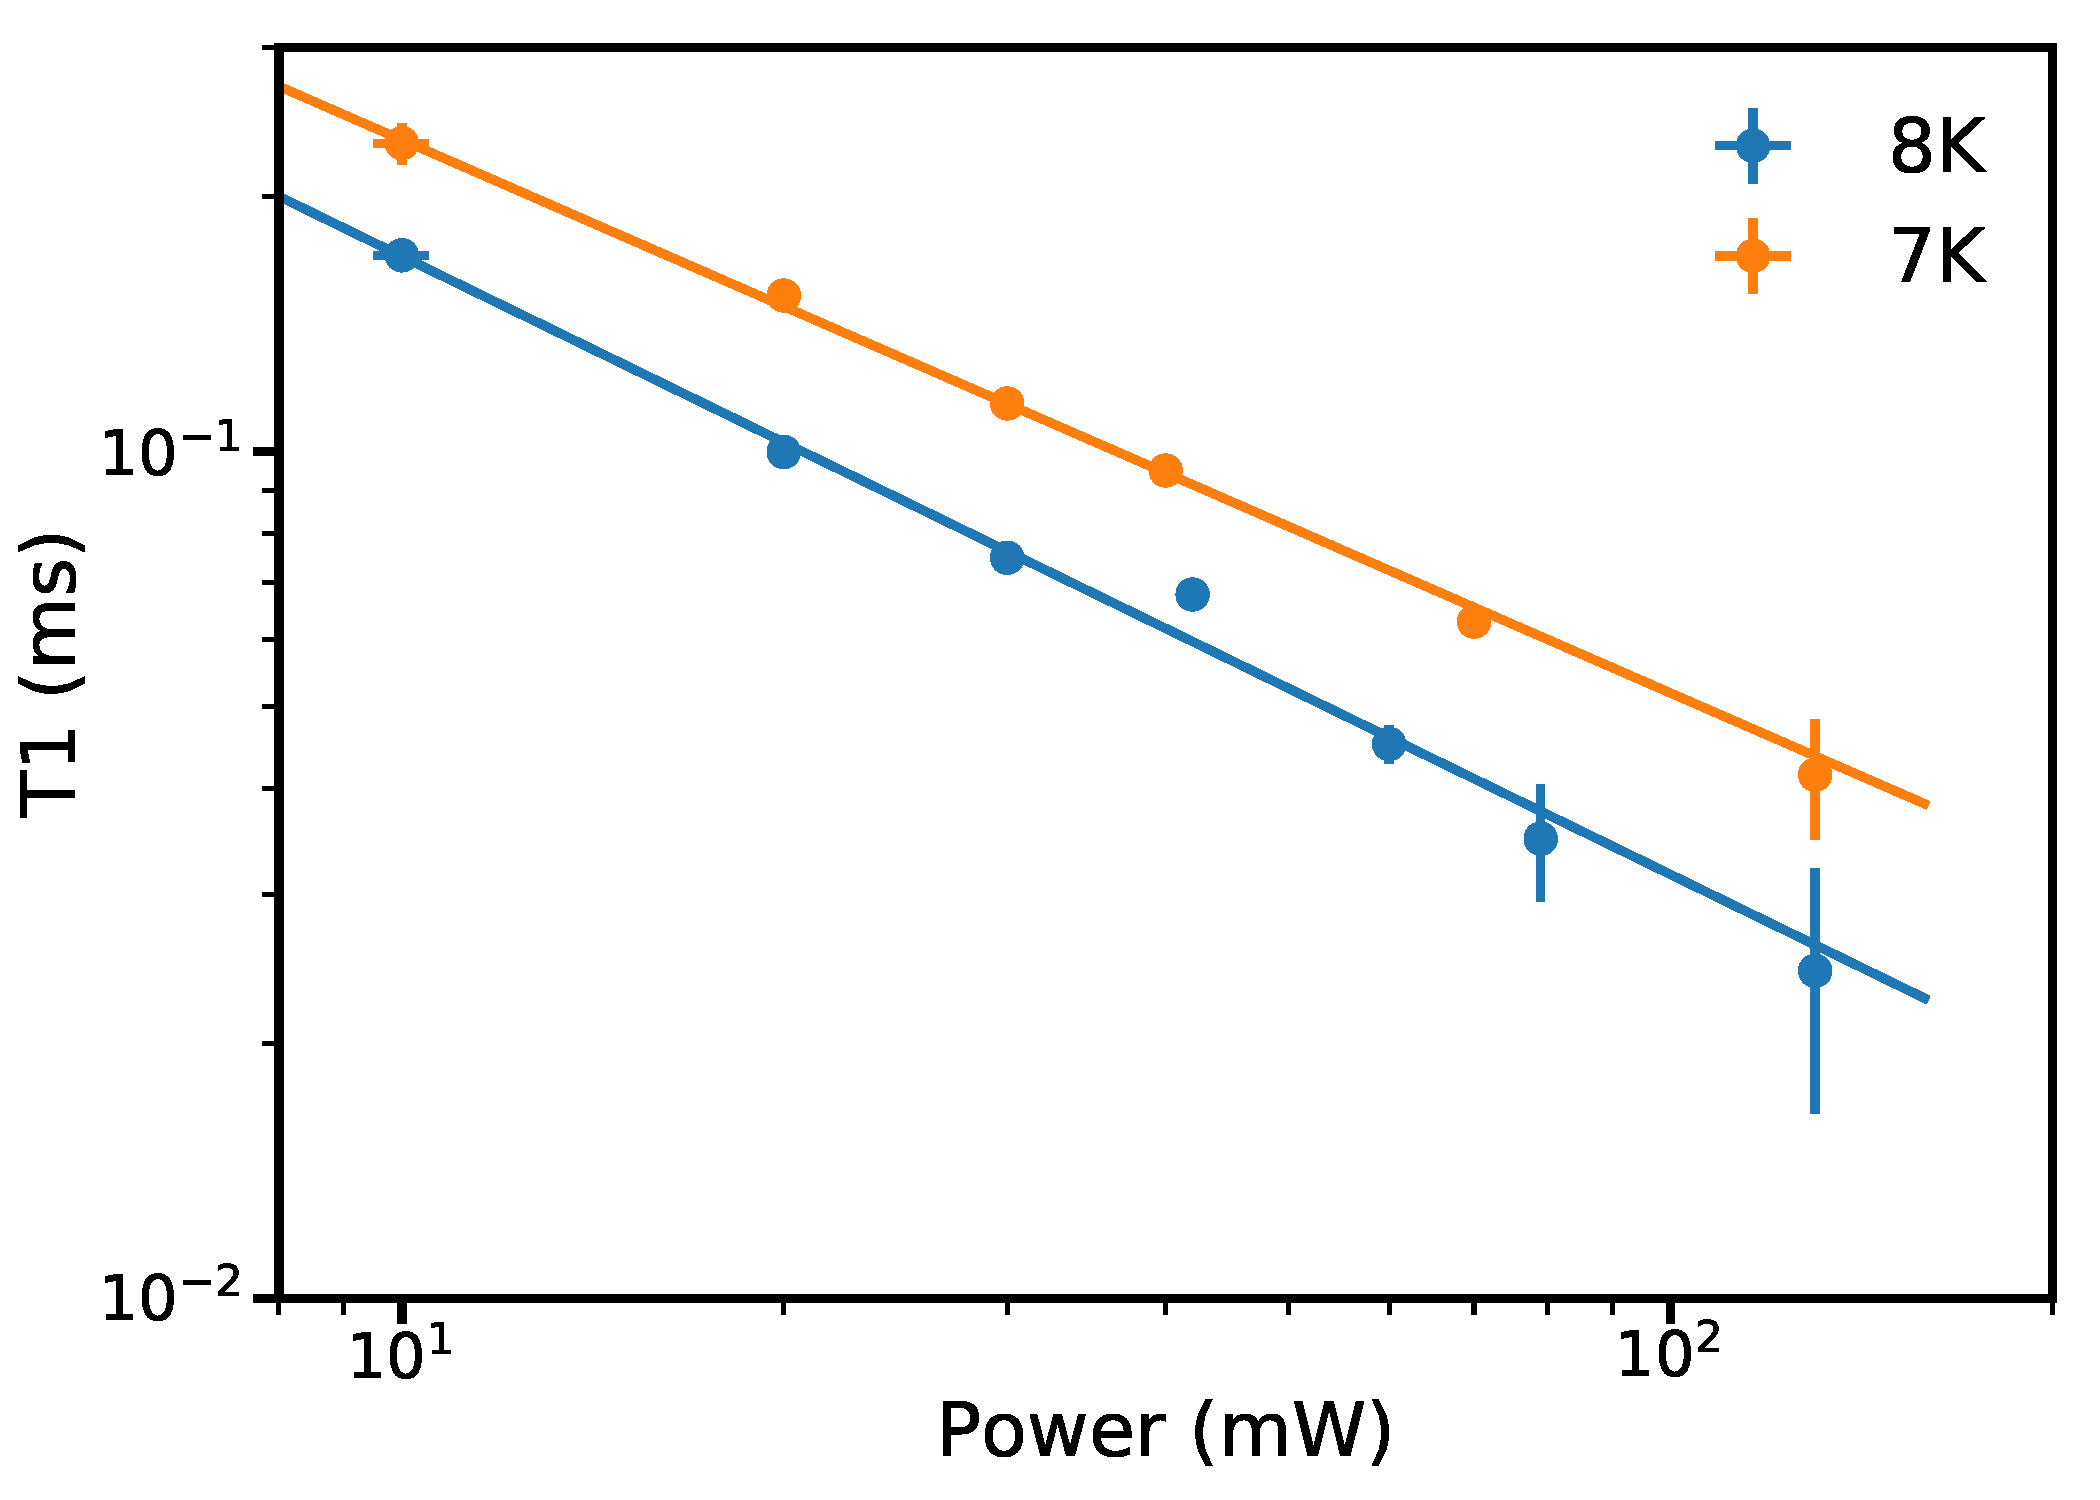
\includegraphics[width=0.8\columnwidth]{Figures/T17Kvs8k_1058nmTest.pdf}
\caption[$T_1$ temperature comparison]{Figure shows how $T_1$ changes with laser power at 1058~nm and for 8~K and 7~k, with respective dark $T_1$s of 2.77~ms and 32.2~ms. It is interesting to note that there is a clear increase in relaxation rate at 8~K vs 7~k. This suggests that the mechanism by which the laser acts has some temperature dependence.}
\label{fig:t1tempcomp}
\end{figure}

What is immediately clear from this comparison is that the laser is not a completely limiting factor - at the same power and wavelength but different temperatures different $T_1$ times are observed.
The 8~K fit has the same parameters as given above, whilst the 7~K fit has a power of $0.65\pm 0.002$.
At 7~K there is a clear increase in $T_1$ at the same laser power relative to 8k, suggesting that whatever mechanism is reducing relaxation time does indeed have a temperature dependence.
I will now address the mechanisms that are potentially responsible for the observed effects, concentrating on heating.

\subsection{Heating as a Mechanism of Relaxation}

Estimating the potential effect of heating as a result of laser illumination is complex.
The first factor affecting such an estimation is that the temperature sensor that is used to control the cryostat is not located on the sample so the highly localised heating caused by a laser would likely not be detected.
Beyond this, estimations are made difficult by the somewhat scarce information on light absorption at cryogenic temperatures in silicon.
The reason that heating is presented as a potential explanation for the observed relaxation effects is the extremely low heat capacity of silicon at cryogenic temperatures, as predicted by the Debye model \cite{ANDP:ANDP19123441404}.
This means that only a small amount of energy is required to effect significant heating in silicon.
Also relevant is that silicon is a poor photo-emitter, meaning that any infra-red radiation absorbed is likely to end up as heat rather than emitted photons.
Calculating potential heat rises is made difficult by the scarcity of literature on the absorption coefficient of silicon at low temperatures.
Studies have concentrated on silicon at room temperature due to its use in solar cells and have tended to assume that low-temperature, below band-gap absorption will be low due to the scarcity of phonons to assist transitions and conduction band electrons to absorb sub band gap photons.
Interest has been peaked recently due to the possibility of taking advantage of the anticipated high transmission qualities of silicon at low temperatures for use as an interferometer in a gravitational wave detector \cite{Degallaix2014}.
One study in particular provides a useful insight, although not a directly comparable one.
This measured the absorbance of silicon at 6~K by monitoring its temperature increase under illumination by a 1550~nm laser.
Results of this experiment show a much greater absorption than anticipated, with the measured result being the same at 6~K as at room temperature: 0.030cm$^{-1}$.
Taking this figure as a guideline, it can be estimated that approximately $0.5\%$ of incident light is absorbed by the sample in these experiments.
Harder to estimate is the rate at which the sample is cooled in the cryostat, which will determine how much extra energy it holds in equilibrium with the laser turned on.
In \cite{Degallaix2014} the sample was observed to increase in temperature as long as the laser was turned on.
It was, however, poorly thermally coupled to its cooling environment and it seems likely that a sample in direct contact with helium flow will reach an equilibrium temperature value.
Here I make the assumption that approximately $1\%$ of the laser power is retained in the sample at equilibrium, adding to its temperature.
This figure can then be used along with heat capacity, taken from \cite{Desai1986,Glazov2001}, to calculate the expected temperature for a given laser power.
Using this temperature along with the equations in section \ref{sec:mechrelax} allows an estimation of $T_1$ and $T_2$ times at given laser powers.
\\
A further potential contributor to relaxation rates is donor ionisation - unpaired electrons on the donor being excited to the conduction band by an incident photon.
This would be registered first as a loss in signal and then a relaxation back to thermal equilibrium as the donor is recaptured by an ionised donor.
This process also contributes to heating of the sample - an electron excited to the conduction band \emph{thermalises} (relaxes to the energy minimum of the conduction band) rapidly - but this effect is already accounted for in the heating calculation.
The cross section for this process is predicted to be small - peaking at $17\times10^{-16}\text{cm}^{-2}$ and significantly smaller at the wavelengths used in these experiments \cite{Sclar1984,Ross2017a}.
Following \cite{Ross2017a}, a figure of $1.5\times10^{-16}\text{cm}^{-2}$ is used to calculate rate of donor ionisation with power.
Given these parameters, a simulation of relaxation rate based on laser power, when accounting for donor ionisation rates and heating effects is given in figure \ref{fig:t1t2sim}.

\begin{figure}
\centering
\begin{subfigure}[b]{\textwidth}
\centering
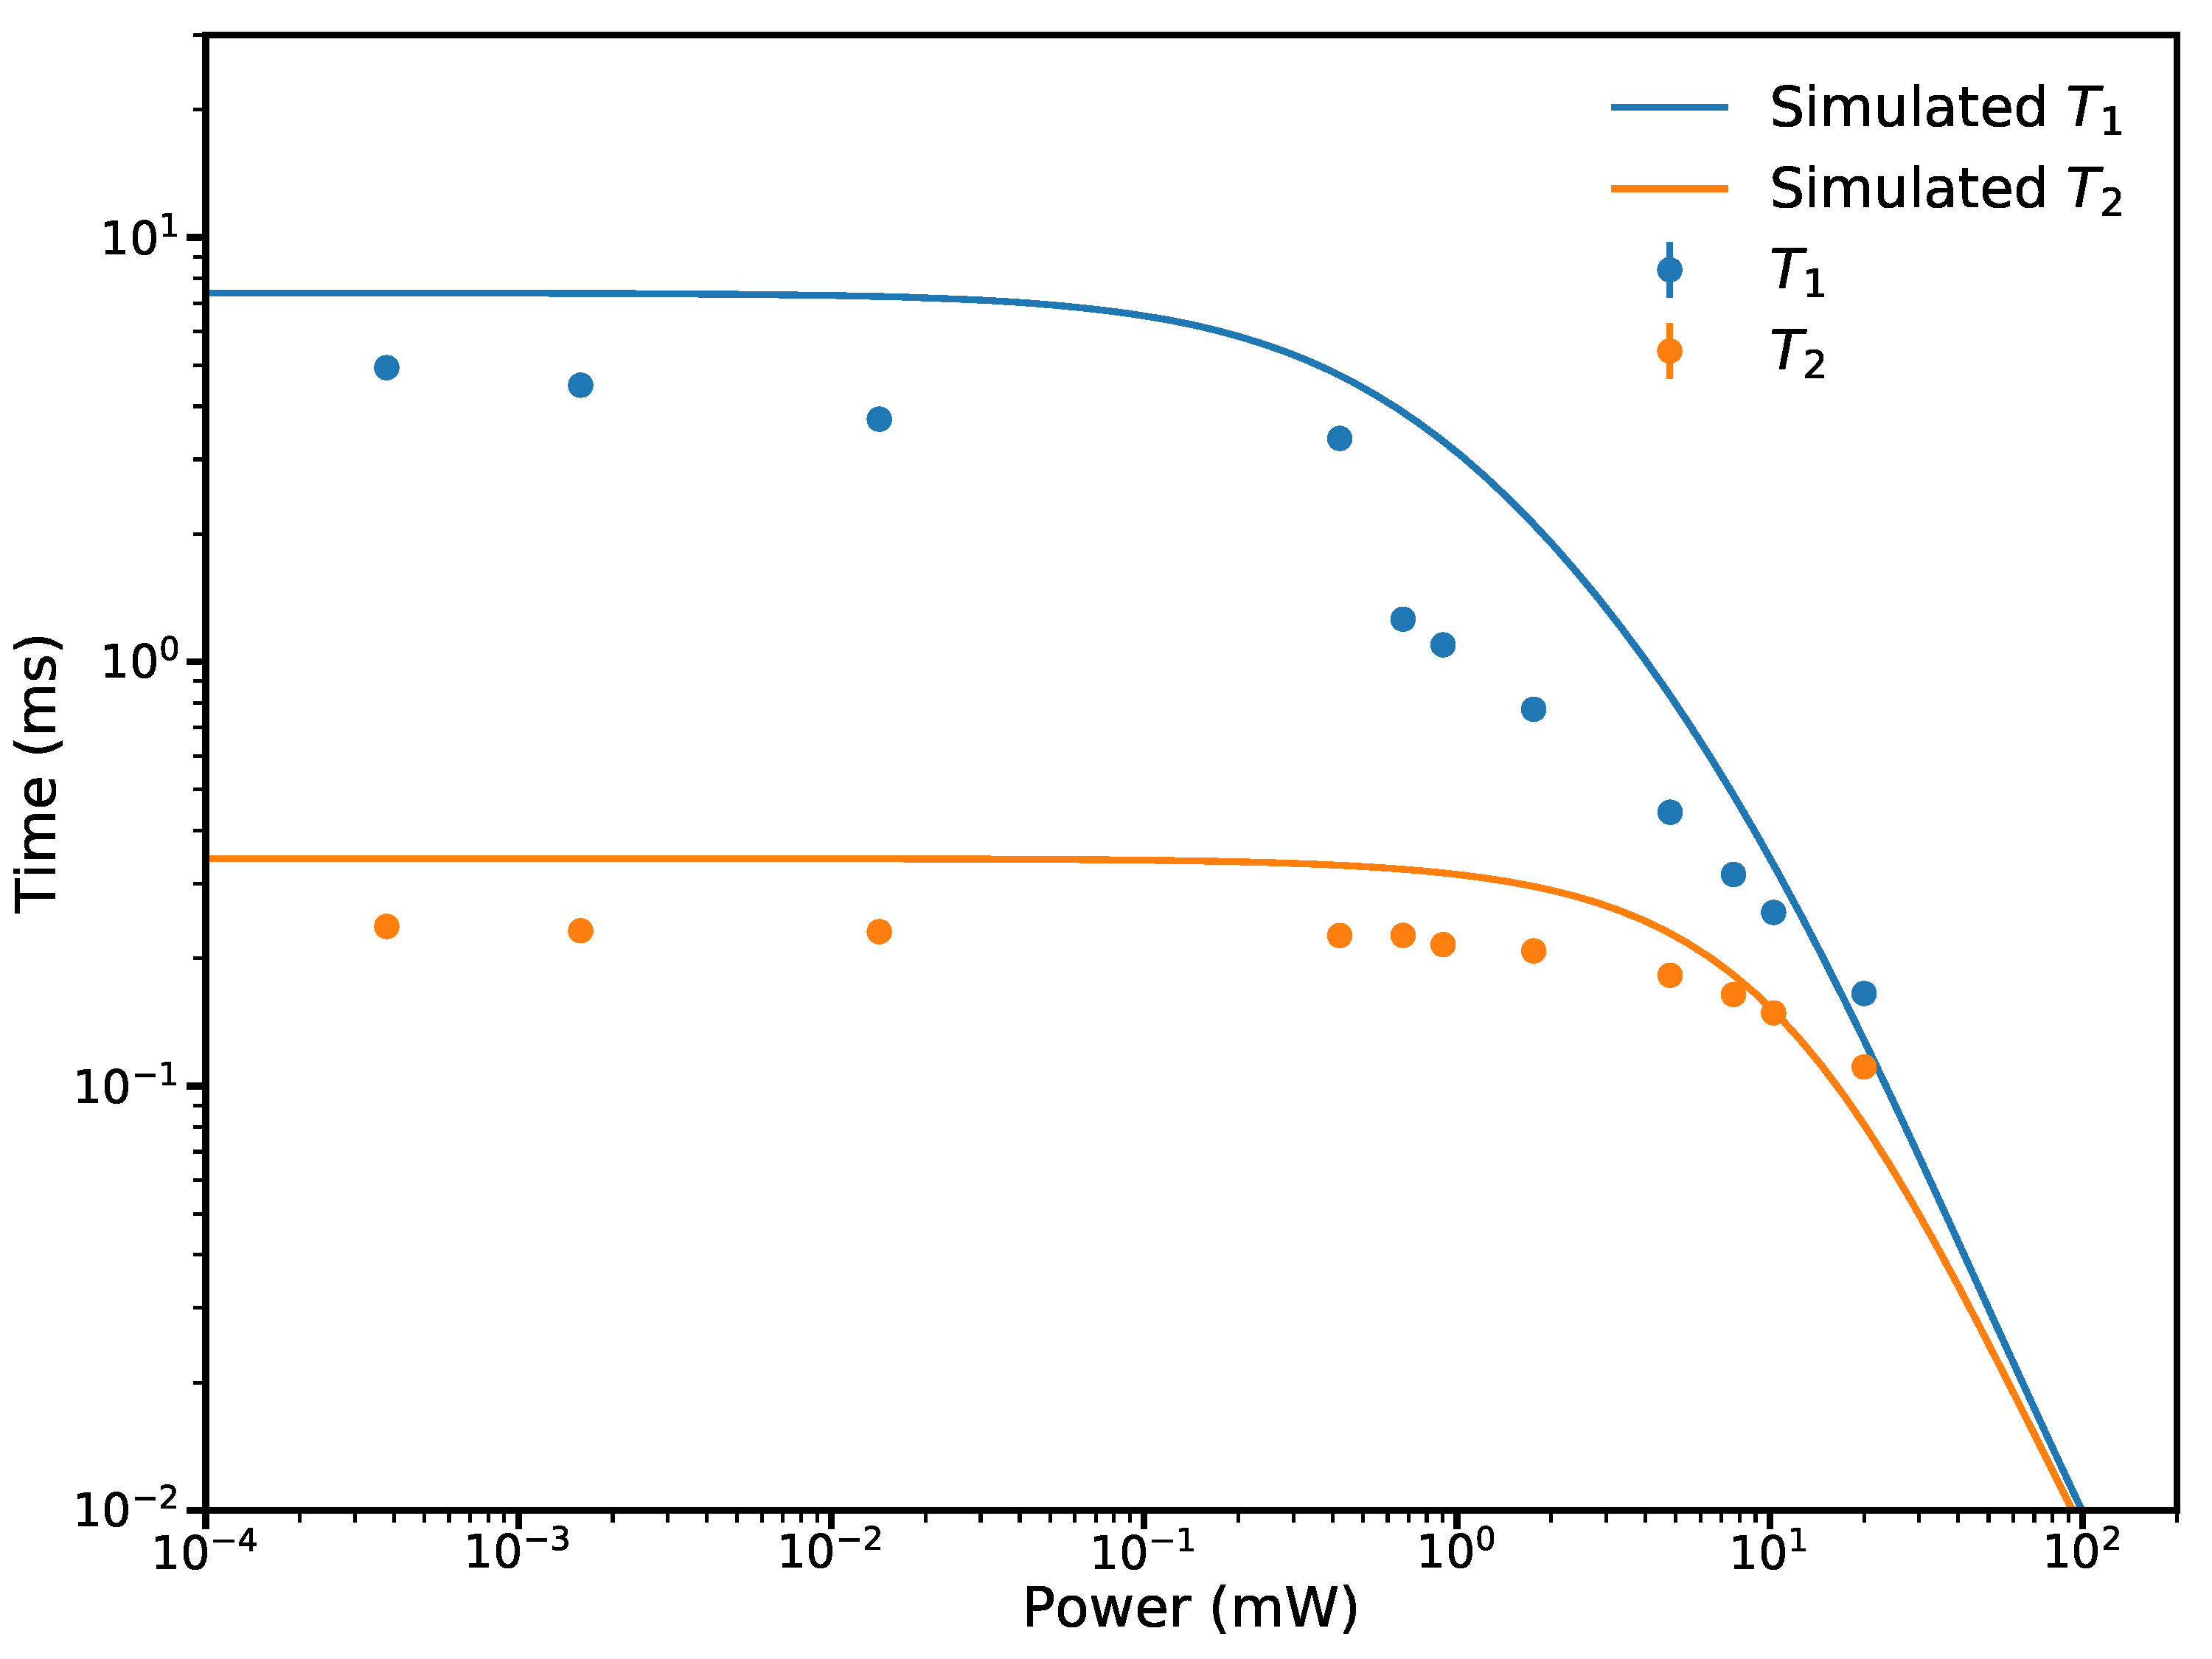
\includegraphics[width = 0.8\columnwidth]{Figures/simt1t2.pdf}{(a)}
\end{subfigure}
\begin{subfigure}[b]{\textwidth}
\centering
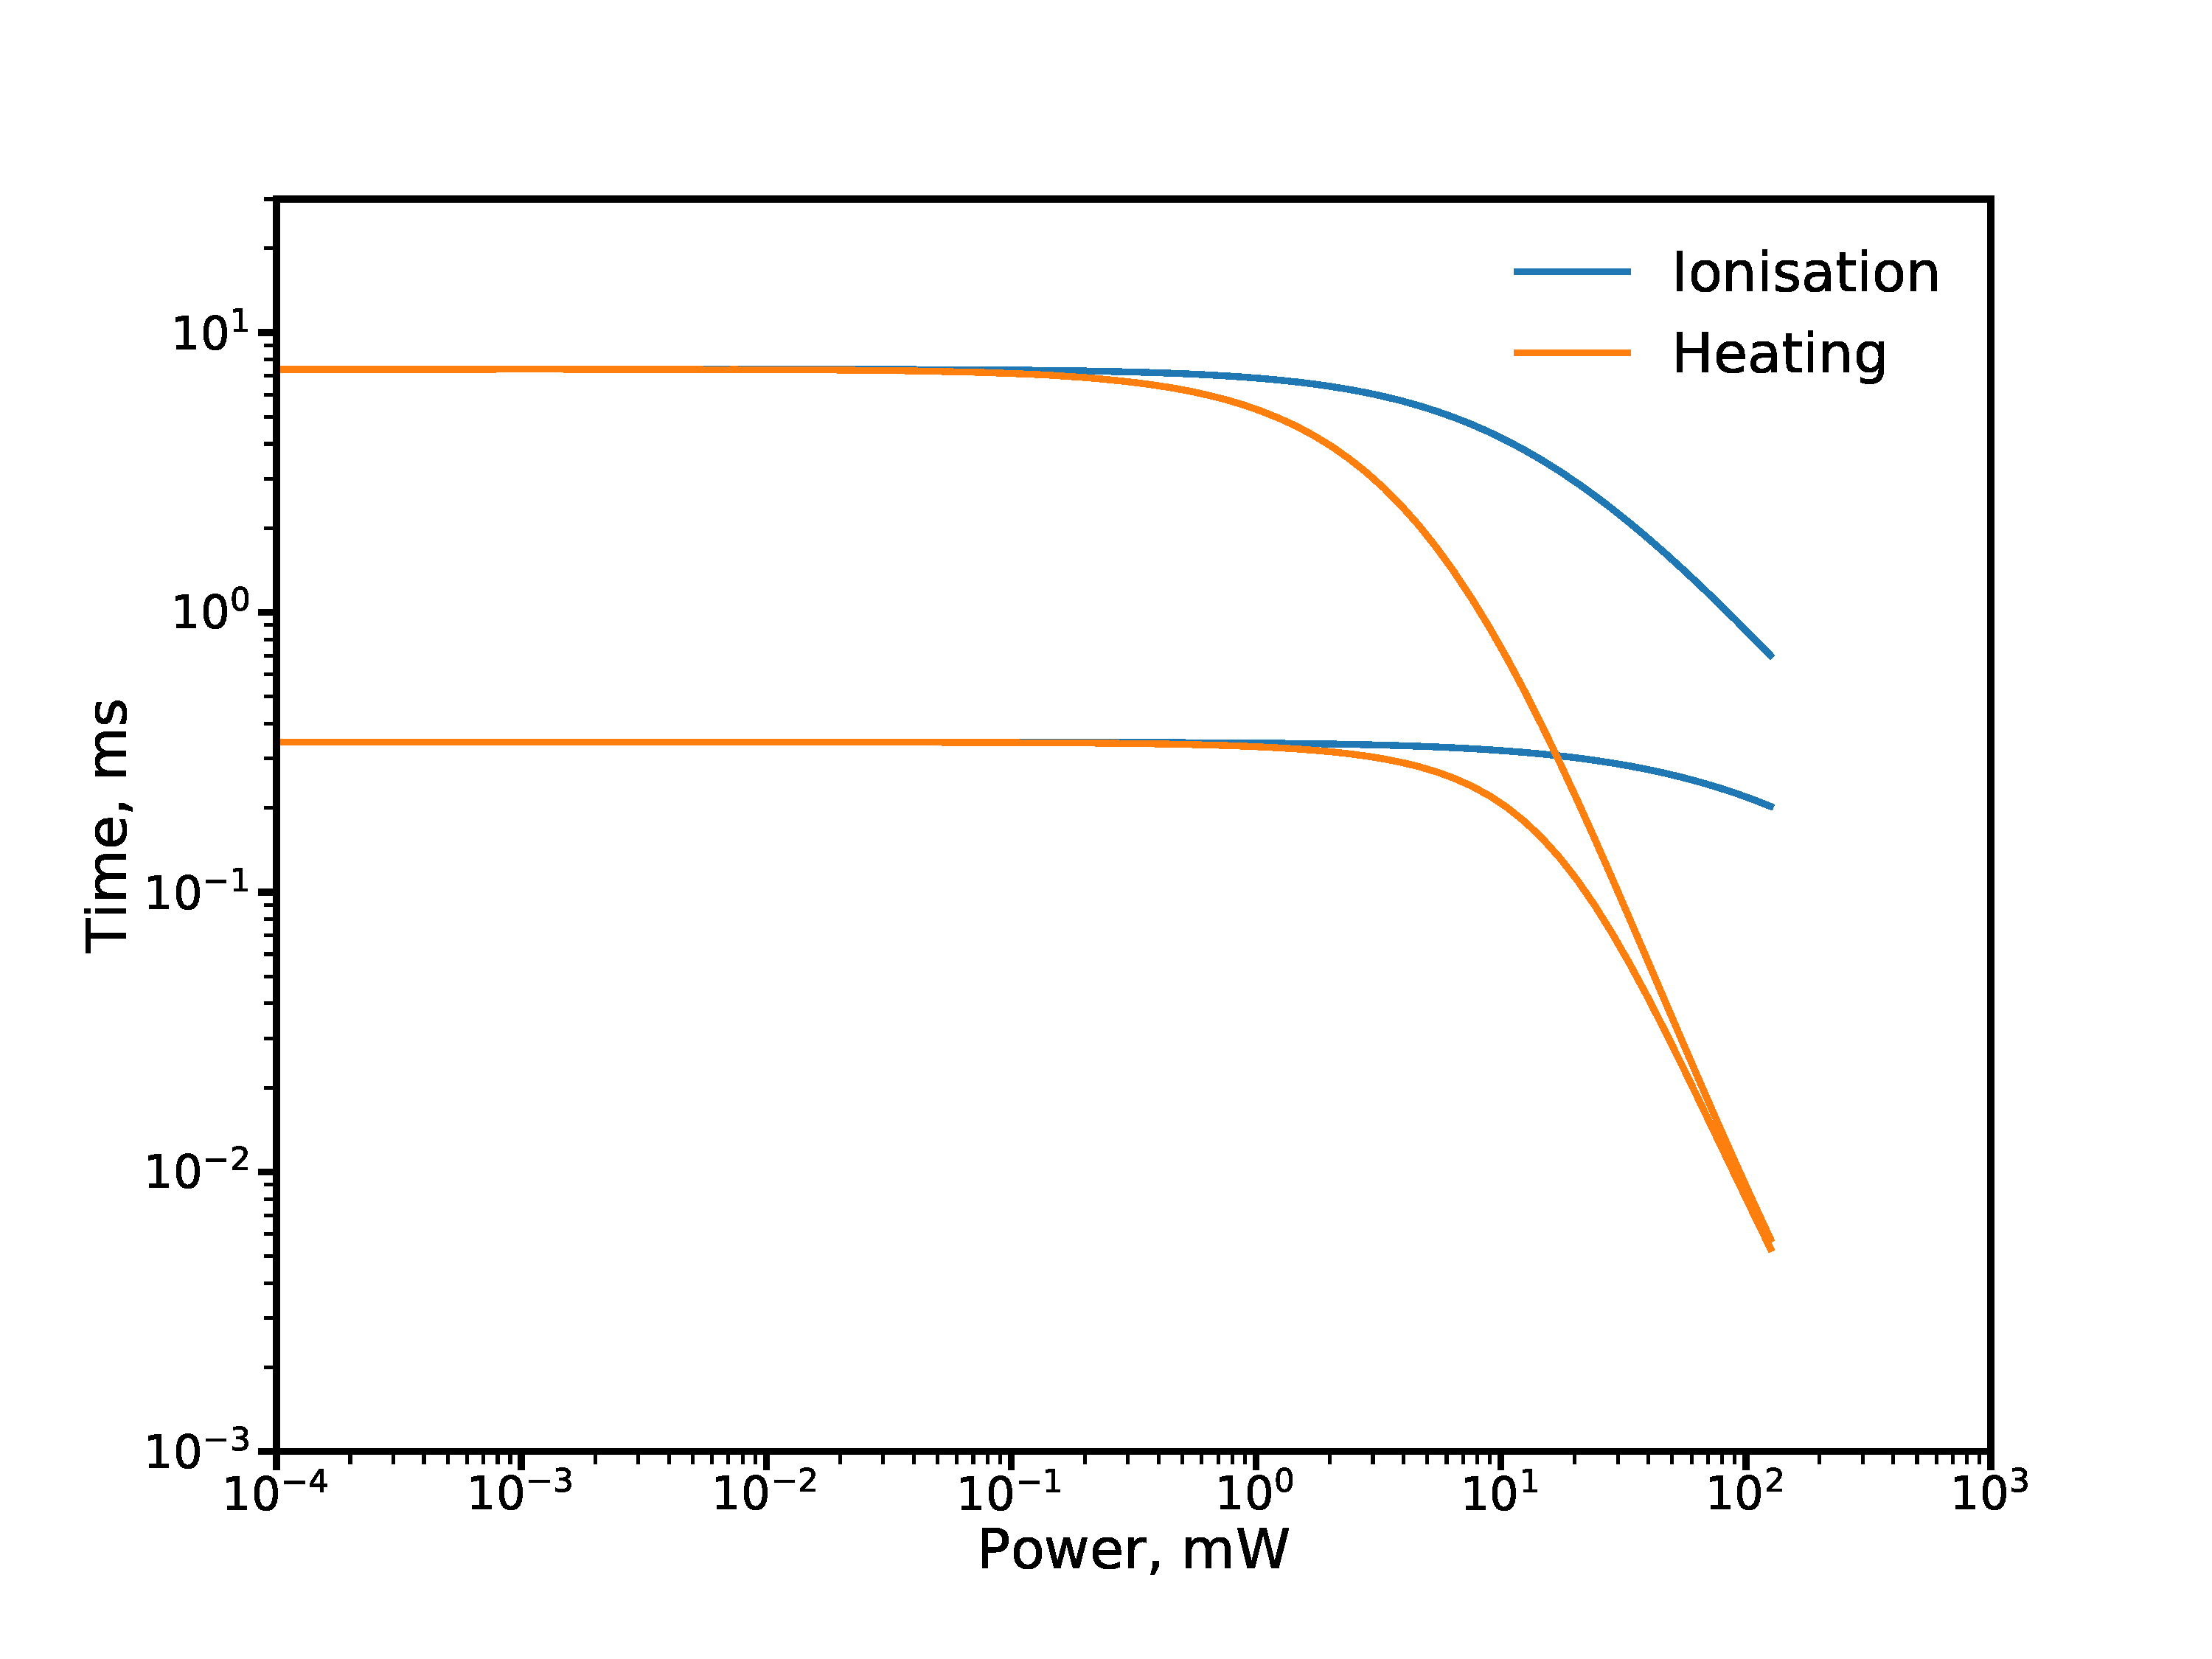
\includegraphics[width = 0.8\columnwidth]{Figures/ionvsheat.pdf}{(b)}
\end{subfigure}
\caption[Simulated $T_1$ under heating]{Figure showing the simulated $T_1$ and $T_2$ as as a function of laser power at 8~K when taking account of potential heating and donor ionisation, alongside low power data taken at the same temperature. \textbf{(a)} shows the combined impact of heating and donor ionisation whilst \textbf{(b)} shows their individual contributions - demonstrating that heating is the apparently dominant effect. Data for $T_1$ and $T_2$ calculated using heat capacity of silicon at these temperatures alongside equations shown in section \ref{sec:mechrelax}, whilst donor ionisation rates use cross sections given in \cite{Sclar1984,Ross2017a}.}
\label{fig:t1t2sim}
\end{figure}

The results shown here, whilst by no means conclusive, suggest that heating is a potential cause of the observed effects.
Some wavelength dependence would also be expected with a heating based mechanism - as the absorbance of the laser light is dependent upon the wavelength.
At higher powers the heating effect appears to increase faster in the simulation than in the experimental results but further work will be required to refine these figures.
Heating does appear to account quite well for the observed discrepancy in $T_1$ and $T_2$ times at each temperature.
\\
I have not discussed the mechanism that Feher and Gere identify as the most prominent in their results: the double spin exchange between free electron, donor electron and donor nucleus.
This process, although mentioned by Feher and Gere, is given no explicit form.
A qualitative argument is used to explain why it accounts for the observed behaviour of electron relaxation time under illumination.
As such it is difficult to incorporate such a mechanism into my simulations.
One question would be whether this mechanism would demonstrate the temperature dependence that has so far been observed, with relaxation occurring more slowly at lower temperatures but under the same illumination.
It is possible that the lower thermal velocity of free electrons at lower temperatures could account for the discrepancy, giving a smaller number of double scattering events per second.
This presents an excellent next step for this work: determining both the density of free carriers at each wavelength and using this to provide an account of the scattering rate of electrons on donors.
